\documentclass{article}

% Language setting
% Replace `english' with e.g. `spanish' to change the document language
\usepackage[english]{babel}
\usepackage{comment}
% Set page size and margins
% Replace `letterpaper' with`a4paper' for UK/EU standard size
\usepackage[letterpaper,top=2cm,bottom=2cm,left=3cm,right=3cm,marginparwidth=1.75cm]{geometry}

% Useful packages
\usepackage{amsmath}
\usepackage{amssymb}
\usepackage{paracol}
\usepackage{graphicx}
\usepackage{subfig}
%\usepackage{subcaption}
\usepackage[colorlinks=true, allcolors=blue]{hyperref}
%
\usepackage{caption}
\title{Impacting model BEB }
\author{Peter}

\begin{document}
\maketitle

\begin{abstract}
Your abstract.
\end{abstract}

\section{Modelling}
For a conservative SDOF impact oscillator, we would like to start from it to know how the Boundary Equilibrium Bifurcation occurs and the condition for its existence and stability. We suppose that there is a external force $\mu$ to change the equilibrium for + region to - region.  
\begin{equation}
 m_0 \ddot{X} + c_0 \dot{X} + k X =f
\end{equation}
Dividing both sides of the equation above (in time T) with $k$ and letting $X_{st}=\frac{f}{k}$, we can get 
\begin{equation}
    \frac{\ddot{X}}{\omega^{2}_0}+\frac{c_0}{k}\dot{X}+X=X_{st}
    \label{eq:2}
\end{equation}
Meanwhile, take the substitution by $ \displaystyle  \rm{d} t= \omega_0 \rm{d} T$,$ \displaystyle  \bar X=\frac{X}{X_{st}}$ and $ \displaystyle 2\xi=\frac{c_0\omega_0}{k}$, sometimes called damping ratio, we can get a nondimensionalized  equation in a general form
\begin{equation}
    \ddot{\bar{X}} +2\xi \dot{\bar{X}}+ \bar{X}=1
    \label{eq:nondim Equi1}
\end{equation} if $f>0$ and 
\begin{equation}
    \ddot{\bar{X}} +2\xi \dot{\bar{X}}+ \bar{X}=-1
     \label{eq:nondim Equi2}
\end{equation} if $f<0$.
where $ \displaystyle \omega_0=\sqrt{\frac{k}{m_0}}$ is the natural frequency of the system.
At $\bar X=0$ the velocity will be reset by an impact map. 

Obviously, the system is an impacting class hybrid system. Before impact the system will be governed by an ODE $\dot x= F(x)$, and  a reset map can be exposed when the state variables get onto the boundary super surface to get the post-impact state. At first, let us guess a more universal piecewise model according to the terms in book [Piecewise-smooth dynamical systems: Theory and applications]. The single impacting face is defined by a smooth function  $H(x)=0$, 
\begin{equation}
    \Sigma =  \{x|H(x)=0\}, \text{and the region}, S^+=\{x|H(x)>0\}; 
\end{equation}
So that we can rearrange the hybrid system in a more canonical form
\begin{align}
    \dot x=F(x) \quad \text{if} \; H(x)>0\\
    x \mapsto R(x) \quad \text{if} \; H(x)=0
\end{align}
Here we introduce some key terms, $\dot{x}^+$ and $\dot{x}^-$ are namely the post- and pre-impact states and the $v(x)$ is so-called normal velocity at which the trajectory governed by $S^+$ approaches the impact manifold, which can be defined by a \textit{Lie derivation}
\begin{equation}
    v(x)=\mathcal{L}_{F}(H)(x)=\frac{dH}{dx} \dot x=H_x F
\end{equation}
meanwhile the $a(x)$ is the acceleration at the boundary,
\begin{equation}
    a(x)=\mathcal{L}^2_{F}(H)(x)=H_{xx} F+H_x F_x F
    \label{eq: normal acceleration definition}
\end{equation}
If an impact law which can make the state follow a grazing trajectory back to itself (when the $v(x)=0$) we can set the \textit{Reset map} as following 
\begin{equation}
    R(x)=x+W(x)v(x)
\end{equation}
where the $W(x) \in \mathbb{R}^n$ is a smooth function.
After the grazing case can be taken into consideration, the surface can be divided into three regions $\Sigma^-=\{x \in \Sigma: v(x)<0\}$, $\Sigma^0=\{x \in \Sigma: v(x)=0\}$, $\Sigma^+=\{x \in \Sigma: v(x)>0\}$. In impacting hybrid systems, there will be usually three cases when the trajectory approaches the $\Sigma$,

$Case I: \rm{abs} (v(x)^-)> \epsilon$ then a simple reset map will be used $x^+ =  x^- + W(x) v(x)^-$

$Case II: \rm{abs}(v(x)^-) < \epsilon \;\text{and} \; a(x)<0$ 
then there another map to  
quickly end the chattering sequence and the trajectory will get into sliding set, and the sticking vector field will be 
\begin{equation}
    \dot x= F_s=F(x)-\lambda (x) W(x) ,\quad \lambda>0
\end{equation}
The rough explanation for the definition[ref nordmark] is that the sliding motion's change in infinitesimal time will be governed by $F(x)$ and an infinitesimal negative impacting velocity in to the boundary, thus $dx=F dt - |u|W$. And the $\lambda$ can be determined by 
\[\lambda(x)=\frac{\mathcal{L}^2_F(H)(x)}{\mathcal{L}_{W} \mathcal{L}_F(H)(x)}=\frac{-a(x)}{1+r(x)}\]

\subsection{$f>0$}
Make translation $U=\bar X-1$, in this case, when the trajectory hits the $\Sigma=\{ U+1=0\}$ the $a(x)>0$ so there is no sticking set.
\begin{equation}
    \ddot U+2\xi \dot U+U=0
    \label{eq:generalized 1dof equation}
\end{equation}
 and now the reset map will take pace at $U=-1$. This model and be depicted by fig.\ref{fig:SDof Model}
 \begin{figure}
     \centering
     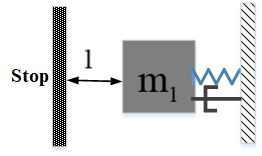
\includegraphics[width= 0.5 \textwidth]{pictures/SDOF_model.png}
     \caption{Sketch of the SDOF impact model}
     \label{fig:SDof Model}
 \end{figure}
 
 And the general solution of the Eq. \ref{eq:generalized 1dof equation} will be
 \begin{align}
     U=e^{-\xi t}\left [U_0\cos{\omega_1 t}+\frac{\dot U_0+\xi U_0}{\omega_1} \sin{\omega_1 t}  \right]\\
     \dot U=e^{-\xi t}\left[ \dot U_0 \cos{\omega_1 t}-\frac{U_0+\xi \dot U_0}{\omega_1} \sin{\omega_1 t}\right]
 \end{align}
 If the trajectory's starting point is $(U_0,\dot U_0)=(-1,S)$, then 
 \begin{align}
     U=e^{-\xi t}\left [-\cos{\omega_1 t}+\frac{S-\xi }{\omega_1} \sin{\omega_1 t}  \right]\\
     \dot U=e^{-\xi t}\left[ S \cos{\omega_1 t}-\frac{\xi S -1}{\omega_1} \sin{\omega_1 t}\right]
 \end{align}
 Suppose that the trajectory will arrive at the $U=-1$ with velocity $S^{'}$ at time $t_1=\frac{\tau_1}{\omega_1}$
 \begin{align}
     -1&=e^{-\mu \tau_1}\left [-\cos{\tau_1}+\frac{S-\xi }{\omega_1} \sin{\tau_1}  \right]\\
    S^{'}&=e^{-\mu \tau_1}\left[ S \cos{\tau_1}-\frac{\xi S -1}{\omega_1} \sin{\tau_1}\right]
 \end{align}
 Where $\displaystyle \mu = \frac{\xi}{\omega_1}=\frac{\xi}{\sqrt{1-\xi^2}}$. Thus, we can get S, $S^{'}$ as a function $\tau_1$
 \begin{align}
     S&=-\frac{e^{\mu \tau_1}-\cos{\tau_1}-\mu \sin{\tau_1}}{\sqrt{1+\mu^2}\sin{\tau_1}} \label{eq: bounding velocity}\\ \nonumber
     S^{'}&=e^{-\mu \tau_1}\left[ (\cos{\tau_1-\mu\sin{\tau_1}})S+\sqrt{1+\mu^2}\sin{\tau_1}\right]\\ \nonumber
     &=e^{-\mu \tau_1} \left[ \frac{-1}{\sqrt{1+\mu^2}\sin{\tau_1}}  (e^{\mu \tau_1}\cos{\tau_1}-\mu e^{\mu \tau_1}\sin{\tau_1}-\cos^2{\tau_1}+\mu \cos{\tau_1}\sin{\tau_1}-\mu \cos{\tau_1}\sin{\tau_1}+\mu^2\sin^2{\tau_1}) \right. \\ \nonumber 
     & +
     \left. \sqrt{1+\mu^2}\sin{\tau_1} \right]\\ \nonumber
     &=\frac{e^{-\mu \tau_1}}{\sqrt{1+\mu^2}\sin{\tau_1}}\left[ -e^{\mu \tau_1}\cos{\tau_1}+\mu e^{\mu \tau_1}\sin{\tau_1}+\cos^2{\tau_1}-\mu^2\sin{\tau_1}+(1+\mu^2)\sin^2{\tau_1}\right]\\
     &=\frac{e^{-\mu \tau_1}-\cos{\tau_1}+\mu \sin{\tau_1}}{\sqrt{1+\mu^2}\sin{\tau_1}}
     \label{eq:hitting velocity}
 \end{align}
 we find that \[ \frac{\rm d S}{\rm d \tau_1}=-\frac{1-e^{\mu \tau_1}(\cos{\tau_1}-\mu\sin{\tau_1})}{\sqrt{1+\mu^2}\sin^2{\tau_1}}
\] and  \[ \frac{\rm d S^{'}}{\rm d \tau_1}= \frac{1-e^{-\mu \tau_1}(\cos{\tau_1}+\mu \sin{\tau_1})}{\sqrt{1+\mu^2}\sin^2{\tau_1}}\]
 We introduce the auxiliary function\cite{ANDRONOV1966443}
 \begin{equation}
     \varphi(\tau,\mu)=1-e^{\mu \tau}(\cos{\tau}-\mu\sin{\tau}), \; \partial \varphi/\partial{\tau}=e^{\mu\tau}(1+\mu^2)\sin{\tau}
 \end{equation}
 \begin{figure}
    \centering
    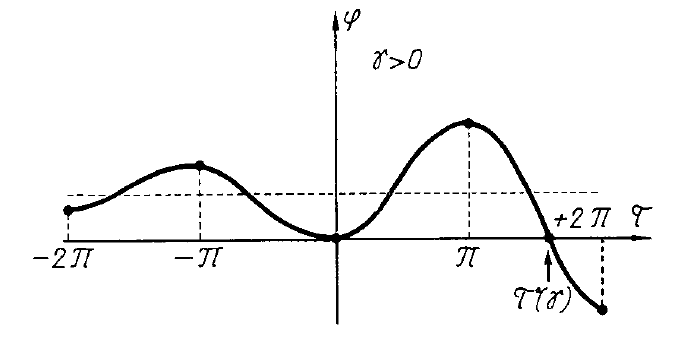
\includegraphics[width=0.6 \textwidth]{pictures/auxiliary_fun.png}
    \caption{auxiliary function}
    \label{fig:auxiliary function}
\end{figure}
Then we can reorganize the equations above to
\begin{subequations} \label{eq: reorganization after aux}
\begin{align}
    S&=-\frac{e^{\mu \tau_1}(1-e^{-\mu \tau_1}(\cos{\tau_1}+\mu \sin{\tau_1}))}{\sqrt{1+\mu^2}\sin{\tau_1}} = -\frac{e^{\mu \tau_1}\varphi(\tau_1,-\mu)}{\sqrt{1+\mu^2}\sin{\tau_1}}  \label{eq: REO S}\\ 
    S^{'}&=\frac{e^{-\mu \tau_1}(1-e^{\mu \tau_1}(\cos{\tau_1}-\mu \sin{\tau_1}))}{\sqrt{1+\mu^2}\sin{\tau_1}}=\frac{e^{-\mu \tau_1}\varphi(\tau_1,\mu)}{\sqrt{1+\mu^2}\sin{\tau_1}}    \label{eq: REO S'} \\
    \frac{\rm d S}{\rm d \tau_1}&=-\frac{\varphi(\tau_1,\mu)}{\sqrt{1+\mu^2}\sin^2{\tau_1}}  \label{eq:REO dSdt} \\
    \frac{\rm d S^{'}}{\rm d \tau_1}&=\frac{\varphi(\tau_1,-\mu)}{\sqrt{1+\mu^2}\sin^2{\tau_1}} \label{eq: REO dS'dt}
\end{align}
\end{subequations}
Thus $S$ is the starting velocity and the $S^{'}$ is the velocity at next intersection point, after some evolution time. Here we consider two different conditions: $(1)f>0$ (admissible equilibrium); $(2)f<0$ (pseudo equilibrium).

\subsubsection{Case I: $\xi>0$}

For simplicity, we suppose $S>0$, from fig.\ref{fig:auxiliary function}  we know that when $S^{'}=0$ there will be two roots of $\tau_1$ namely $\tau_1^1=0$ and $\tau_1^2=\tau(\mu)\in (\pi,2\pi)$. The non-trivial root $\tau_1^2$ stands for the evolution time. Using Eq.\ref{eq: REO S} we can get the critical value for \[S_{cr}=-\frac{e^{\mu \tau(\mu)}\varphi(\tau(\mu),-\mu)}{\sqrt{1+\mu^2}\sin{\tau(\mu)}}\]

It means that when $S<S_{cr}$ the path will eventually be attracted to the origin and only those cases with larger S will have the chance to hit the boundary $U=-1$ and continue the evolution loop.
 \begin{equation} 
 S=S_{cr}+\int_{\tau(\mu)}^{\pi}\frac{\rm d S}{\rm d \tau_1} \rm d \tau_1
 \label{eq:intS}
 \end{equation}
According to eq.\ref{eq:REO dSdt} we can get eq.\ref{eq:intS} and obviously when $\tau_1$ varies from 0 to $\pi$, S will vary from 0 to $-\infty$ and vary from 0 to $+\infty$ when $\tau_1$ varies from $\tau(\mu)$ to $\pi$; in another word,
\begin{align}
    \lim_{S \rightarrow S_{cr}+}\tau_1&=\tau(\mu)^-, \; \lim_{S \rightarrow +\infty}\tau_1=\pi^+ 
    \label{eq:admissible eq evolution}
    \\
    \lim_{S \rightarrow -0}\tau_1&=0^+,\;\lim_{S \rightarrow -\infty}\tau_1=\pi^-
    \label{eq:pseudo eq evolution}
\end{align}

In our case, we assume that the path of this system starts with a positive velocity S and arrives the boundary $U=-1$ with a negative velocity $S^{'}$, and obviously the relationship between the $S$ and $S^{'}$ is implicitly defined by the eq.\ref{eq: reorganization after aux}. However, based on $\displaystyle |\frac{\rm d S^{'}}{\rm d S}|=\frac{\varphi(\tau_1,-\mu)}{\varphi(\tau_1,\mu)}>0$ and, $\tau_1 \in (\pi,\tau(\mu))$ with initial point $S^{'}(0)=0,\;S=S_{cr}$. As $S\rightarrow+\infty$, there will be an asymptotic result
%

\begin{align}
&\lim_{S \rightarrow +\infty}\ |\frac{S^{'}}{S}|=\lim_{\tau_1\rightarrow \pi^+} |-e^{-2\mu\tau_1}\frac{\varphi(\tau_1,\mu)}{\varphi(\tau_1,-\mu)}|=\lim_{\tau_1\rightarrow \pi^+} |-e^{-2\mu\tau_1}e^{\mu \pi}|= e^{-\mu \pi}\\
&\lim_{S \rightarrow +\infty} |S^{'}|-e^{-\mu \pi}S=e^{-\mu \pi}
\label{eq: asymptotic line}
\end{align}
%
and 
\begin{align}
  \nonumber
  \frac{|\rm d S^{'}/\rm d S|}{\rm dS}=\frac{\rm d \frac{\varphi(\tau_1,-\mu)}{\varphi(\tau_1,\mu)}} {\rm d \tau_1} \frac{1}{\rm d S/\rm d \tau_1}\\ 
  = \frac{2(1+\mu^2)^{\frac{3}{2}} \sin^3{\tau_1} (\sinh{\mu \tau_1} - \mu \sin{\tau_1})}{\phi^3(\tau_1,\mu)}<0
\end{align}
\begin{figure}[htbp]
    \centering
    \subfloat[$0<\xi<1$]{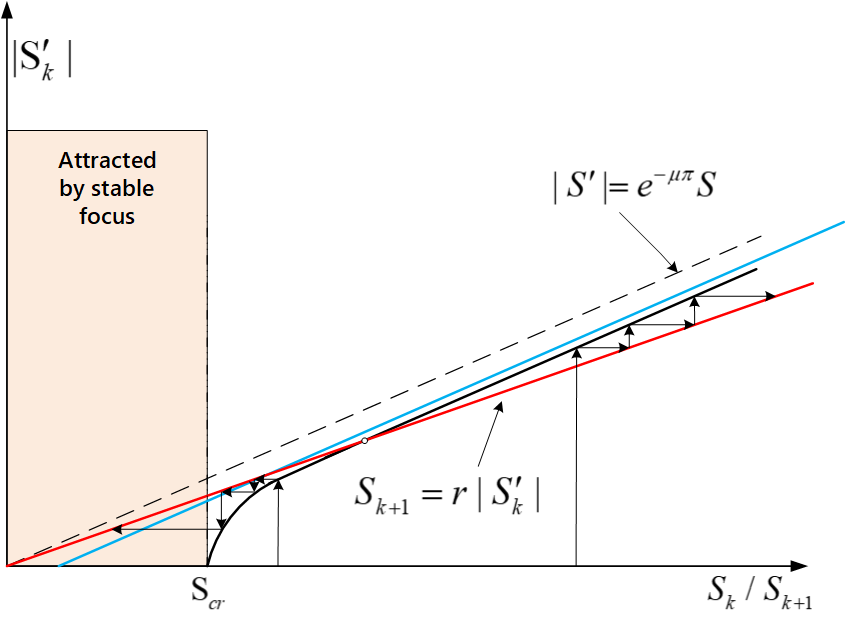
\includegraphics[height=0.3 \textheight, width = 0.5 \textwidth]{pictures/SDOF_impact_S.png}
    }
    \quad
    \subfloat[$\xi=0$]{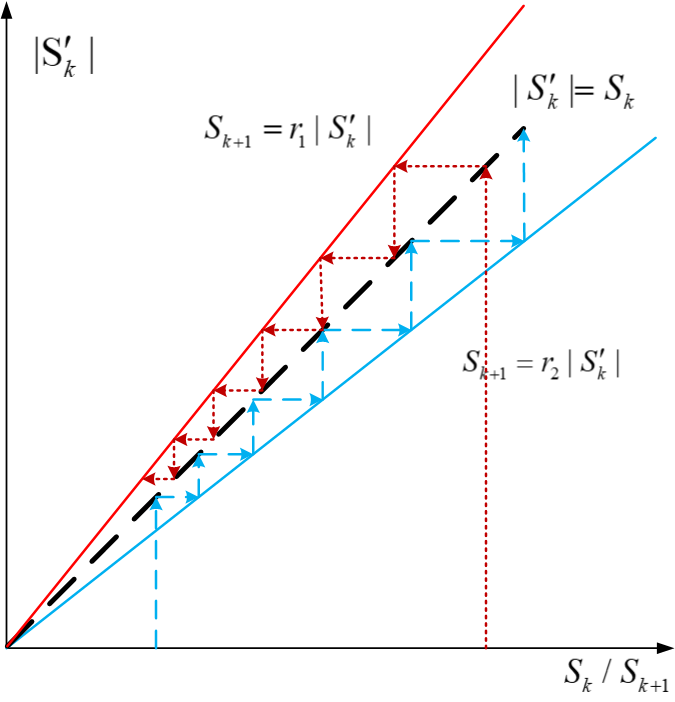
\includegraphics[width = 0.45 \textwidth]{pictures/SDOF_impact_mu0.png}
    }
    \quad
    \subfloat[$\xi<0$]{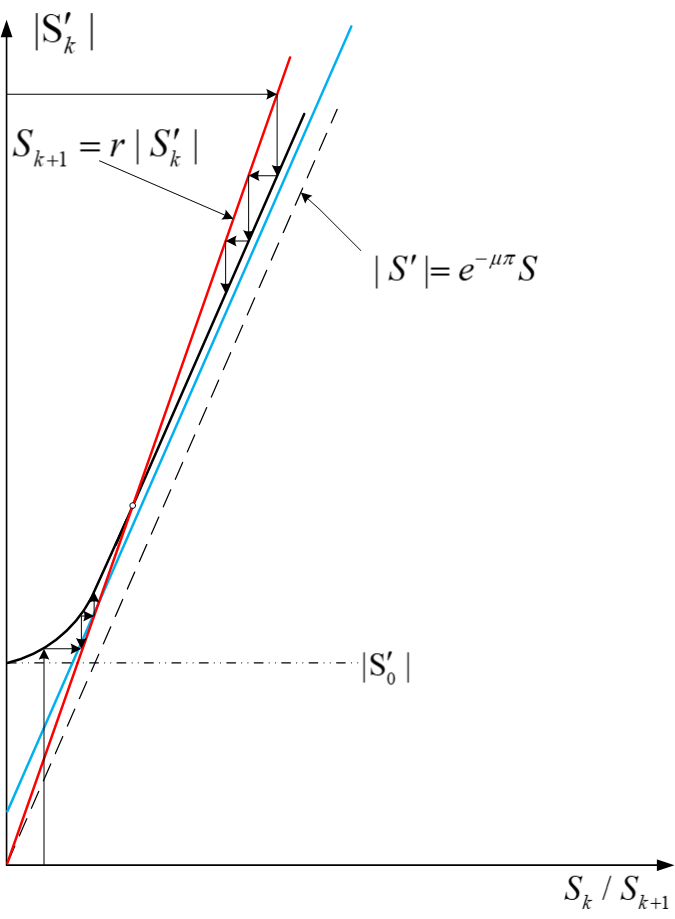
\includegraphics[width = 0.45 \textwidth]{pictures/SDOF_impact_US.png}
    }
    \caption{Three cases : $I:\,0<\xi<1;\;II:\,\xi=0;\;III:\,\xi<0$}
    \label{fig:three cases for mu}
\end{figure}
Thus we have a map $S_0\rightarrow S^{'}_0=-P_0*S_0 \rightarrow S_1=-r*S^{'}_0=r*P_0*S_0\rightarrow S^{'}_2=-P_1*S_1\rightarrow ...$. We can plot this map fig.\ref{fig:three cases for mu}.a. It can be seen that there is no stable limit cycle.

\subsubsection{Case II: $\xi<0$}


In this case,  given a bounding velocity, the return time $\tau_1$ will be given, $S^{'}>S>0$ due to the divergent motion.  $S=0$ is the critical value and the $\tau(\mu)$
is solved by eq.\ref{eq: REO S}, which is easily shown the same as the result in the previous case. Substitute the $\tau(\mu)$ into eq.\ref{eq: REO S'} we can get $S^{'}_{cr}$. And the asymptotic's slope is the same expression as in eq.\ref{eq: asymptotic line}. The impact map is still $S_{k+1}=-rS^{'}_{k}$, and the composed map will be the fig.\ref{fig:three cases for mu }. It shows that if and only if $1/r>e^{-\mu \pi}$ will there be a limit cycle and even globally stable.
\subsubsection{Case III: $\xi=0$}

Interesting enough, in this case, the equilibrium is right located on the boundary, and  $re^{\mu pi}$ means there will be LCO with any amplitude, $r<1$ will lead to convergence to a LCO with amplitude 1 and $r>1$ will lead to divergent motion.

\subsection{$f<0$}
\section{2DOF coupling impacting oscillator}
Based on the SDOF impacting oscillator, adding another object to the previous model by tuning the coupling term leads to another bifurcation analysis.
\begin{equation}
\begin{bmatrix} m_{11} & m_{12}\\ m_{21},&m_{22}
\end{bmatrix} \begin{bmatrix}
\ddot{X_1}\\ \ddot{X_2}
\end{bmatrix}+\begin{bmatrix} c_{11} & c_{12}\\ c_{21}& c_{22}
\end{bmatrix} \begin{bmatrix}
\dot{X_1}\\ \dot{X_2}
\end{bmatrix}+\begin{bmatrix} k_{11} & k_{12}\\ k_{21}&k_{22}
\end{bmatrix} \begin{bmatrix}
X_1\\ X_2
\end{bmatrix}=\begin{bmatrix}
f_1\\0
\end{bmatrix}
\end{equation}
%
multiply both sides with diagonal mass matrix's inversion, we can get
\begin{equation}
\begin{bmatrix} 1 & \frac{m_{12}}{m_{11}}\\ \frac{m_{21}}{m_{22}}&1
\end{bmatrix} \begin{bmatrix}
\ddot{X_1}\\ \ddot{X_2}
\end{bmatrix}+\begin{bmatrix} \frac{c_{11}}{m_{11}} & \frac{c_{12}}{m_{11}}\\ \frac{c_{21}}{m_{22}}& \frac{c_{22}}{m_{22}}
\end{bmatrix} \begin{bmatrix}
\dot{X_1}\\ \dot{X_2}
\end{bmatrix}+\begin{bmatrix} \frac{k_{11}}{m_{11}} & \frac{k_{12}}{m_{11}}\\ \frac{k_{21}}{m_{22}}& \frac{k_{22}}{m_{22}}
\end{bmatrix} \begin{bmatrix}
X_1\\ X_2
\end{bmatrix}=\begin{bmatrix}
\frac{f_1}{m_{11}}\\0
\end{bmatrix}
\end{equation}
%
Using transformation $ \omega_0^2=\frac{k_{11}}{m_{11}},\rm{d} t= \omega_0 \rm{d} T, \frac{m_{22}}{m_{11}}=\gamma ,\frac{\omega_2}{\omega_1}=\eta  $ and dividing both sides with $\omega_0^2$ we can get $X_{st}=\frac{f}{k_{11}},\xi_1=\frac{1}{2}\frac{c_{11}}{m_{11} \omega_0}$ and
\begin{equation}
\begin{bmatrix} 1 & \gamma m_c\\ m_c &1
\end{bmatrix} \begin{bmatrix}
\ddot{X_1}\\ \ddot{X_2}
\end{bmatrix}+\begin{bmatrix} 2 \xi_1 &  \gamma c_c\\ c_c & 2 \xi_2 \eta
\end{bmatrix} \begin{bmatrix} 
\dot{X_1}\\ \dot{X_2}
\end{bmatrix}+\begin{bmatrix} 1 & \gamma k_c\\ k_c & \eta^2
\end{bmatrix} \begin{bmatrix}
X_1\\ X_2
\end{bmatrix}=\begin{bmatrix}
\frac{f_1}{k_{11}}\\0
\end{bmatrix}
\end{equation}
Non-dimensionalizing the displacement by $X_{st}$ leads to $U_1=\frac{X_1}{X_{st}},U_2=\frac{X_2}{X_{st}}$. Meanwhile, setting the non-diagonal part of the matrix as perturbation using a parameter $\epsilon$, we can get
\begin{equation}
M
\begin{bmatrix}
\ddot{U_1}\\\ddot{U_2}
\end{bmatrix}+ C \begin{bmatrix}
\dot{U_1}\\\dot{U_2}
\end{bmatrix}+K\begin{bmatrix}
U_1\\U_2
\end{bmatrix}=\begin{bmatrix}
1 \\0
\end{bmatrix}
\label{eq:coupling pertubed equation}
\end{equation}
where $M=\begin{bmatrix}
1&0\\0&1
\end{bmatrix}+\epsilon \begin{bmatrix}
0& \gamma m_c\\ m_c& 0
\end{bmatrix}$,$C=\begin{bmatrix}
2 \xi_1&0\\0&2 \eta \xi_2
\end{bmatrix}+\epsilon \begin{bmatrix}
0& \gamma c_c\\ c_c& 0
\end{bmatrix}$,$K=\begin{bmatrix}
1&0\\0&\eta^2
\end{bmatrix}+\epsilon \begin{bmatrix}
0& \gamma k_c\\ k_c& 0
\end{bmatrix}$
using the same impact condition in the previous section with SDOF model and under the same initial conditions $U_1(0)=0;\dot{U_1}(0)=1;U_2(0)=0;\dot{U_2}(0)=1;$, here the $\epsilon$  standing different coupling level, a steady response diagram is got as fig.\ref{fig:2DOF_diagram}.
%
\begin{figure}[htpb]
    \centering
    \subfloat[eigenvalue]{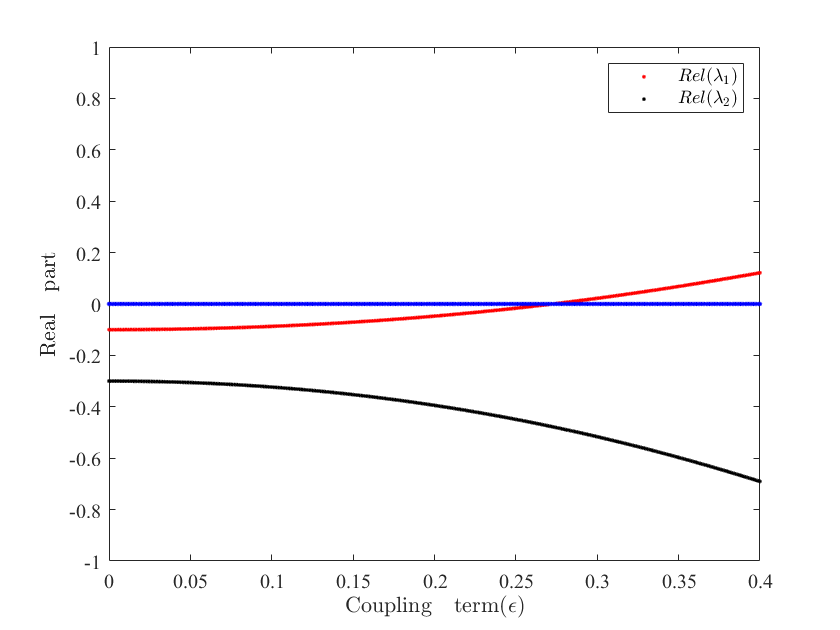
\includegraphics[width =0.5 \textwidth]{pictures/2Dof_eigen_value.png}}
    \quad
    \subfloat[m1 steady peak velocity]{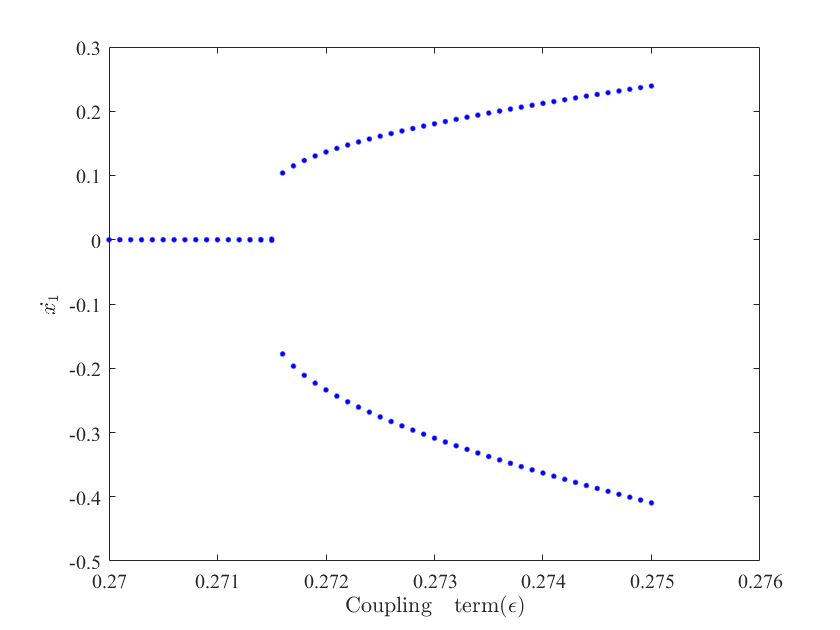
\includegraphics[width =0.5 \textwidth]{pictures/2Dof_m1_diagram.png}}
    \quad
    \subfloat[m2 steady peak velocity]{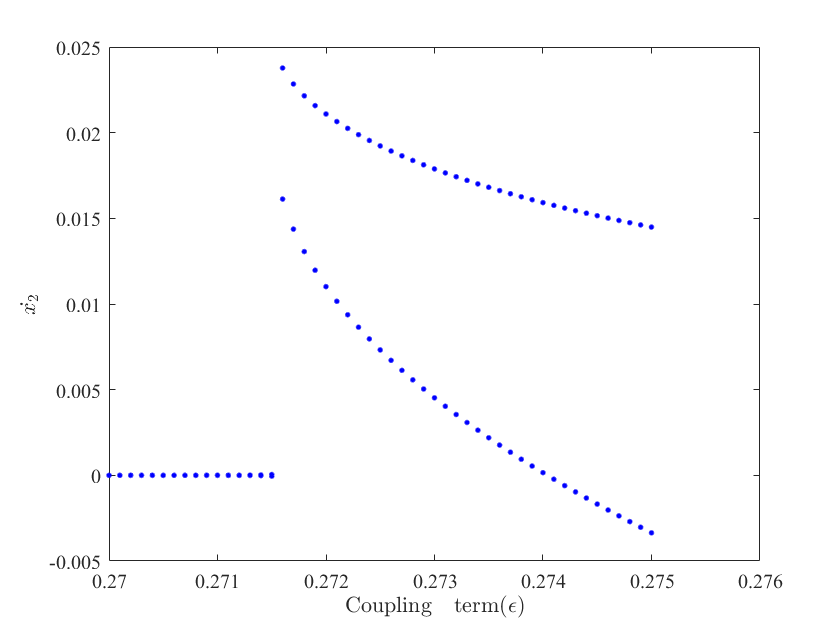
\includegraphics[width =0.5 \textwidth]{pictures/2Dof_m2_diagram.png}}
    \label{fig:2DOF_diagram}
    \caption{2DOF coupled system bifurcation}
\end{figure}
%
\subsubsection{Numerical analysis}
set the $\dot x=F(x)$ with state variables $x=[U_1,U_2,\dot U_1,\dot U_2]$; and the $F(x)=[A]x+b$, where the $A=\begin{bmatrix} 0 & I\\ -M^{-1}K& -M^{-1}C \end{bmatrix}$ and $H(x)=U_1$. $H_x=[1,0,0,0],H_{xx}=\mathbf{0}_{4,4}$. According to the Eq.\ref{eq: normal acceleration definition} we can get \begin{align}
    \nonumber
    F_x&=\begin{bmatrix}
    0 & 0 & 1 & 0\\
    0 & 0 & 0 & 1\\
    0 & 0 & 0 & 0\\
    0 & 0 & 0 & 0
    \end{bmatrix} \\ 
    a(x)&= H_x F_x F\\ \nonumber
    &=\ddot{U_1}
\end{align}and $W(x)=\begin{bmatrix}
0\\ 0\\-1\\m_c 
\end{bmatrix}(1+r)$. Solving this problem will use event-detecting method in code. When $v(x)<\epsilon$ and $a(x)<0$ there will be a chattering sequence and then to a sticking point. And a map $Q(x)$ will be imposed as
\begin{align}
    x^*&=Q(x)=x+\frac{1}{1-r(x)}\left(\frac{2F(x)}{a(x)} r(x) +W(x)\right)v(x)+\mathcal{O}v(x)^2\\
    \Delta t^*&=q(x)=\frac{1}{1-r(x)}\left(\frac{2}{a(x)} r(x) \right)v(x)+\mathcal{O}v(x)^2
\end{align}
The sliding vector field will be \[F_s= F+\frac{a(x)}{1+r(x)}W(x)\]
\subsubsection{Boundary equilibrium bifurcation}
When $f$ changes from negative to positive, the equilibrium will firstly be a pseudo equilibrium ($f<0$), then boundary equilibrium ($f=0$), finally to an unstable admissible equilibrium ($f>0$). The results can be show in Fig.\ref{fig:SDOF BEB} 
\begin{figure}[htpb]
    \centering
    \includegraphics[width= 0.6 \textwidth]{pictures/SDOF_BEB.eps}
    \caption{Boundary equilibrium bifurcation}
    \label{fig:SDOF BEB}
\end{figure}
The amplitude's linear dependence on $\mu$ can be easily  explained by rescaling in Eq.\ref{eq:nondim Equi1} and Eq.\ref{eq:nondim Equi2}. 

For simplicity, we choose $f=1$ for the coupling 2DOF model by adding non-diagonal terms in M, C, K. Suppose there is a limit cycle of $U_1^0(t)$ with period $T_0$, after perturbed with small $\varepsilon$, a new solution $U_1(t)=U_1^0+\epsilon U_1^1$ and $U_2=U_2^0+\epsilon U_2^1$ with period $T=T_0+\epsilon T_1$.
\begin{align}
    U_1^0(t)=A_{10}e^{a_1 t}\cos(\omega_1 t +\phi_1)\\
    \dot{U}_1^0(t)=A_{10}e^{a_1 t}(a_1 \cos(\omega_1 t +\phi_1)-\omega_1 \sin(\omega_2 t+\phi_1))
\end{align}
which satisfy the conditions
\begin{align}
    U_1^0(0)&=0,\; U_1^0(T_0)=0\\
    \dot{U}_1^0(0)&=S_1^0, \; -r \dot{U}_1^0(T_0)=\dot{U}_1^0(0)
    \label{eq: LCO condition}
\end{align}
Correction function $U_1^1$ and $U_2^1$ can be found in \hyperref[Appendix I]{Appendix I}. The $T_0$ is solved by  Eq.\ref{eq: bounding velocity} and Eq. \ref{eq:admissible eq evolution}.
\begin{align}
    U_1(0)&=U_1^0(0)+\epsilon U_1^1(0) \vspace{1em} \\ \nonumber \label{eq: U1 T}
    U_1(T)&=U_1^0(T_0+\epsilon T_1)+\epsilon U_1^1(T_0+\epsilon T_1) \\  \nonumber 
    &= U_1^0(T_0)+\epsilon \dot{U}_1^0(T_0)T_1+\epsilon(U_1^1(T_0)+\dot{U}_1^1(T_0)\epsilon T_1)\\
    &=U_1^0(T_0)+\epsilon(\dot{U}_1^0(T_0)T_1+U_1^1(T_0))+ o (\epsilon)\\  \label{eq: V1 0}
    \dot{U}_1(0)&=\dot{U}_1^0(0)+\epsilon \dot{U}_1^1(0)   \\ \nonumber
    \dot{U}_1(T)&=\dot{U}_1^0(T_0+\epsilon T_1)+\epsilon \dot{U}_1^1(T_0+\epsilon T_1)\\ \nonumber
    &=\dot{U}_1^0(T_0)+\epsilon \ddot{U}_1^0(T_0)T_1+\epsilon(\dot{U}_1^1(T_0)+\ddot{U}_1^1(T_0)\epsilon T_1)\\ \label{eq: V1 T}
    &=\dot{U}_1^0(T_0)+\epsilon(\ddot{U}_1^0(T_0)T_1+\dot{U}_1^1(T_0))+ o (\epsilon)
\end{align}
And now, the known terms are $U_1^0(t)$, $T_0$.From Eq. \ref{eq: U1 T} we can get 
\begin{equation}
    \dot{U}_1^0(T_0)T_1+U_1^1(T_0)=0,\; {\color{red}\boxed{\color{black}T_1=-\frac{U_1^1(T_0)}{\dot{U}_1^0(T_0)}}}
    \label{eq: Period correction}
\end{equation} 
In order for the existence of new LCO after perturbation, the condition $-r\dot{U}_1^0(T_0)=\dot{U}_1^0(0)$ should be maintained. Based on Eqs. \ref{eq: V1 0},\ref{eq: V1 T} and \ref{eq: LCO condition}
we can get \[-r(\ddot{U}_1^0(T_0)T_1+\dot{U}_1(T_0))=\dot{U}_1^1(0)\]
further, with Eq.\ref{eq: Period correction} substituted, the above equation becomes 
\begin{equation}
   {\color{red} \boxed{ \color{black} -r(-U_1^1(T_0) \boxed{\frac{\ddot{U}_1^0(T_0)} {\dot{U}_1^0}} +\dot{U}_1^1(T_0))=\dot{U}_1^1(0)}}
  %
\end{equation}
For $U_2$ we suppose once the unknown $\boxed{A_{20}} $and $\boxed{\phi_2}$ , which determine the $U_2^0$, are given and satisfy the following conditions
\begin{align}
    \label{eq: U2 0}
    U_2(0)&=U_2^0(0)+\epsilon U_2^1(0)\\ \nonumber 
    U_2(T)&=U_2^0(T_0+\epsilon T_1)+\epsilon U_2^1(T_0+\epsilon T_1)\\ \nonumber
    &=U_2^0(T_0)+\epsilon \dot{U}_2^0(T_0)T_1 +\epsilon U_2^1(T_0)+\epsilon^2 \dot{U}_2^1(T_0)T_1\\  \label{eq: U2 T}
    &= U_2^0(T_0)+\epsilon(\dot{U}_2^0(T_0)T_1 + U_2^1(T_0))+o(\epsilon)\\ \label{eq: V2 0}
    \dot{U}_2(0)&=\dot{U}_2^0(0)+ \epsilon \dot{U}_2^1(0)\\  \nonumber \dot{U}_2(T)&=\dot{U}_2^0(T_0+\epsilon T_1)+\epsilon \dot{U}_2^1(T_0+\epsilon T_1)\\ \label{eq: V2 T}
    &=\dot{U}_2^0(T_0)+\epsilon(\ddot{U}_2^0 T_1+\dot{U}_2^1(T_0))+o(\epsilon)
\end{align}
Here if $U_2$ is a LCO with period $T$, then from $U_2(0)=U_2(T)$ with Eqs. \ref{eq: U2 0} and \ref{eq: U2 T} we can get 
\begin{align}
     {\color{red} \boxed{ \color{black} U_2^0(0)=U_2^0(T_0)}}\\
    {\color{red} \boxed{ \color{black}U_2^1(0)=\dot{U}_2^0(T_0)T_1+U_2^1(T_0)=0 }}
\end{align}

from $\dot{U}_2(0)=\dot{U}_2(T)-\epsilon m_c (\dot{U}_1(0)-\dot{U}_1(T))$ with Eqs.\ref{eq: V2 0} and \ref{eq: V2 T} we can get
\begin{align}
    \dot{U}_2(0)-\dot{U}_2(T)&=\left( \dot{U}_2^0(0)-\dot{U}_2^0(T_0)\right)+\epsilon \left(\dot{U}_2^1(0)-\ddot{U}_2^0(T_0)T_1-\dot{U}_2^1(T_0)\right)+o(\epsilon)\\
    \dot{U}_1(0)-\dot{U}_1(T)&=\left( \dot{U}_1^0(0)-\dot{U}_1^0(T_0)\right)+\epsilon \left(\dot{U}_1^1(0)-\ddot{U}_1^0(T_0)T_1 -\dot{U}_1^1(T_0)\right)+o(\epsilon)
\end{align}
%
and respectively
\begin{align}
     \label{eq: init compiliance}
    {\color{red}\boxed{ \color{black}\dot{U}_2^0(0)-\dot{U}_2^0(T_0)=-\epsilon m_c\left( \dot{U}_1^0(0)-\dot{U}_1^0(T_0)\right)}}\\ \label{eq: pert compliance}
    \dot{U}_2^1(0)-\ddot{U}_2^0(T_0)T_1-\dot{U}_2^1(T_0)=-\epsilon m_c \left(\dot{U}_1^1(0)-\ddot{U}_1^0(T_0)T_1 -\dot{U}_1^1(T_0)\right)
\end{align}
If we solve $A_{20}$ and $\phi_2$ and the results automatically satisfy the equation Eq. \ref{eq: pert compliance}, then we can say  a new LCO is built in this system??

\begin{figure}
    \centering
    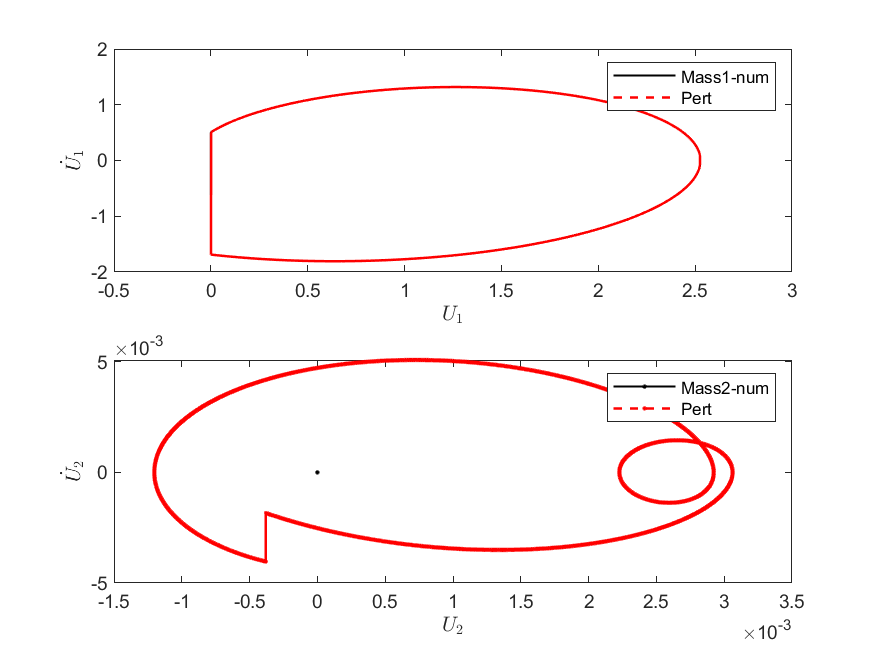
\includegraphics[width = 0.8 \textwidth]{pictures/2DOF_coupling_Pert.eps}
    \caption{Perturbed phase portrait with $\epsilon=0.001$}
    \label{fig:2DOF Pert }
\end{figure}
\section{Airfoil model with freeplay nonlinearity}

Here we introduce a 2-D airfoil model with free-play in the flap hinge. And we simplify the flap motion as impact when colliding with the main body. In this model, $H(x)=\delta^2-\beta^2$,  $x=[\zeta,\alpha,\beta,\dot{\zeta},\dot{\alpha},\dot{\beta},w_1,w_2]^T$. 
\[H_x=[0,0,-2\beta,0,0,0,0,0]\] and \[H_xF=H_x[
\dot{\zeta},\dot{\alpha},\dot{\beta},\ddot{\zeta},\ddot{\alpha},\ddot{\beta},\dot{w_1},\dot{w_2}]^T=-2\beta \dot{\beta}\]
and \begin{align}
    a(x)&=\mathcal{L}_{L}^2(H)(x)\\&=\frac{\partial}{\partial x}(\mathcal{L}_F(H)(x))F\\&=[0,0,-2\dot{\beta},0,0,-2\beta,0,0]F
\end{align}
% 
In this form of $H(x)$ the function $W(x)$ will take this form
\begin{equation}
    W(x)=\frac{1+r}{-2\beta}\begin{bmatrix}
    0\\0\\0\\C_{\zeta}\\C_{\alpha}\\-1\\0\\0
    \end{bmatrix}
\end{equation}
where $\displaystyle C_{\zeta}=\frac{m_{22} m_{13}-m_{12} m_{23}}{m_{11}m_{22}-m_{12}^2}$ and $\displaystyle C_{\alpha}=\frac{m_{11} m_{23}-m_{12} m_{13}}{m_{11}m_{22}-m_{12}^2}$. 


This hybrid system's revolution process can be constructed by a composed map 
\[
\Phi=\varphi\left(y_{0}, T(y_0)\right) \circ R \] ,  where $R \rightarrow y^{+}=P \cdot y^{-}$, $\varphi(x, t) $  is flow in linear region or $ \Phi=R \circ \varphi\left(y_{0}, T\left(y_{0}\right)\right)$. And
$\varphi (y_{0}, T(y_{0})=E(y_{0}) \cdot S(T(y_{0}))$, $\quad S(T (y_{0}))=\left[e^{\lambda_{1} T}, \ldots, e^{\lambda_{2} T}\right]^{\top}$,$E(y_{0})=V \cdot \operatorname{diag}(V^{-1} \cdot y_{0}) \quad(E_{n \times n})$

If there is any LCO, it means that
\[\Phi\left(y^{*}\right)=y^{*}, \quad\left|y^{*}\right|>0\]


\begin{figure}[htbp]
    \centering
    \subfloat[flap degree]{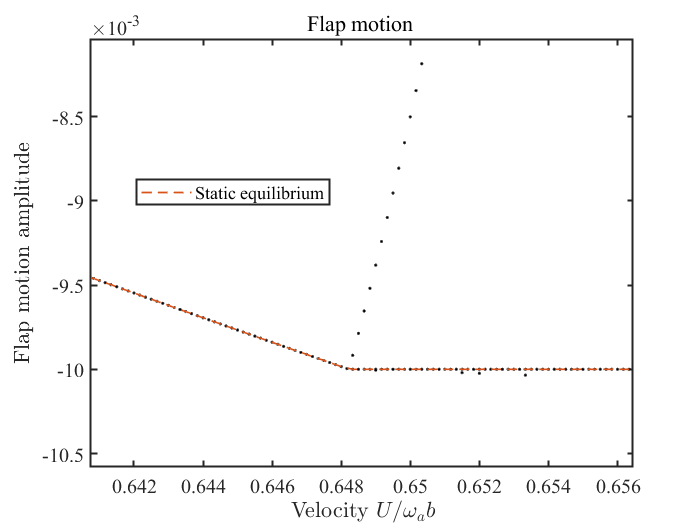
\includegraphics[width =0.5 \textwidth]{pictures/flap_bifurcation.png}}
    \subfloat[heave motion]{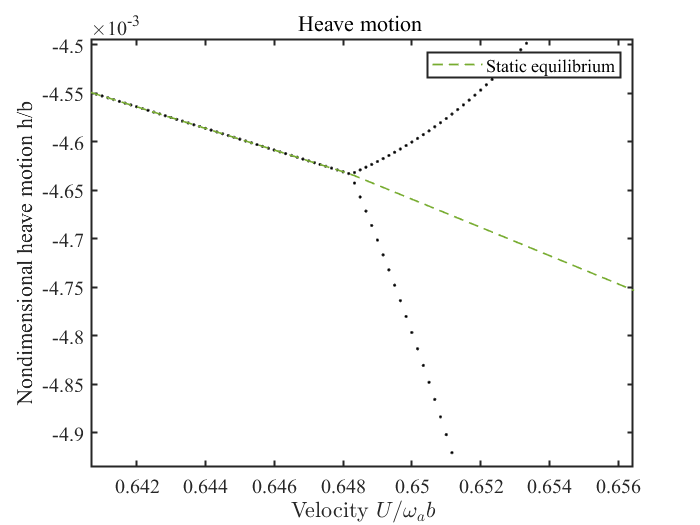
\includegraphics[width =0.5 \textwidth]{pictures/heave_bifurcation.png}}
    \label{fig:3DOF airfoil diagram}
    \caption{ BEB bifurcation}
\end{figure}
%

\appendix
\renewcommand{\theequation}{\Alph{section}.\arabic{equation}}
\renewcommand{\thesubsection}{\Alph{section}.\arabic{subsection}}
\renewcommand{\thesubsubsection}{\Alph{section}.\arabic{subsection}.\arabic{subsubsection}}
\renewcommand{\thefigure}{\Alph{section}.\arabic{figure}}
\renewcommand{\thetable}{\Alph{section}.\arabic{table}}
\clearpage

\section{Appendix I} 
\setcounter{table}{0}
\setcounter{equation}{0}
\label{Appendix I}
Here we give proof of the perturbed solution.
If $U(t)=Ae^{a t}\cos(\omega t+\phi)$. From Eq.\ref{eq:coupling pertubed equation} we can get
\begin{align}
    \ddot{U}_1+\epsilon  \gamma m_c \ddot{U}_2 +2 \xi_1 \dot{U}_1+\epsilon \gamma c_c \dot{U}_2+U_1+\epsilon \gamma k_c U_2=1\\
    \epsilon m_c \ddot{U}_1 + \ddot{U}_2 + 2 \xi_2 \eta \dot{U}_2+\epsilon c_c \dot{U}_1+\eta^2 U_2+\epsilon k_c U_1=0
\end{align}
and $U_1^0=A_{10} e^{a_1 t}\cos(\omega_1 t+ \phi_1)$

$U_2^0=A_{20} e^{a_2 t}\cos(\omega_2 t + \phi_2)$

If we substitute the $U_1=U_1^0+\epsilon U_1^1$ and $U_2^1=U_2^0+\epsilon U_2^1$ into the coupling differential function, and balance the $\epsilon$ terms with different order. we can get the 
\begin{align}
    \ddot{U}_1^1+2 \xi_1 \dot{U}_1^1+U_1^1=- \gamma (m_c \ddot{U}_2^0+c_c \dot{U}_2^0+k_c U_2^0)\\
    \ddot{U}_2^1+2 \eta \xi_2 \dot{U}_2^1+\eta^2 U_2^1= -(m_c \ddot{U}_1^0+c_c \dot{U}_1^0+k_c U_1^0)
\end{align}
Using the given solutions of $U_1^0$ and $U_2^0$ we can get a more simplified form of equation
\begin{align}
    \ddot{U}_1^1+2 \xi_1 \dot{U}_1^1+U_1^1=M_1 e^{a_2 t} \cos(\omega_2 t+\phi_2) +M_2 e^{a_2 t}\sin(\omega_2 t+\phi_2)=F_1(t)\\ \label{eq: correction U21}
    \ddot{U}_2^1+2 \eta \xi_2 \dot{U}_2^1+\mu^2 U_2^1= N_1 e^{a_1 t}\cos(\omega_1 t+\phi_1)+N_2 e^{a_1 t} \sin(\omega_1 t +\phi_1)=F_2(t)
\end{align}
where $$ M_1=A_{20}\gamma ((\eta^{2} \omega_{1}^{2} -a_2^2) m_c -a_{2} c_c -k_c);~M_2=A_{20} \gamma \eta (2 \omega_{1} a_{2} m_c+\omega_{1} c_c)$$
and
$$N_1=A_{10} ((\omega_1^2 - a_1^2) m_c-a_1 c_c-k_c);~N_2=A_{10}(\omega_1 a_1 m_c+\omega_1 c_c)$$ 

$a_1=-\xi_1,a_2=-\xi_2 \eta, \omega_1=\sqrt{1-\xi_1^2}, \omega_2= \eta \sqrt{1-\xi_1^2}$



So we can know the $U_1^1$ and $U_2^1$ can be obtained from the above equations

\[U_1^1(t)=\int_0^t U_1^0(t-\tau) F_1(\tau) \rm{d}\tau\] and \[U_2^1(t)=\int_0^t U_2^0(t-\tau) F_2(\tau) \rm{d}\tau\] or using parameter variation method:
\begin{align}
    %\nonumber
    U_2^1&=v_1(t) Y_1(t) +v_2(t) Y_2(t)%\\
    %&=v_1(t)e^{a_2 t}\cos(\omega_2 t)+v_2(t)e^{a_2 t}\sin(\omega_2 t)
\end{align}
$Y_1$ and $Y_2$ are the basic solutions of homogeneous differential equation governing the second DOF, namely $$\displaystyle Y_1=e^{(a_2+i\omega_2)t}$$ and $$Y_2=e^{(a_2-i\omega_2)t}$$ According to the Book (Peter.D.Miller, Asymptotic analysis, Ch.VII),
$$\dot{U}_2^1=\dot{v}_1(t) Y_1(t) +\dot{v}_2(t) Y_2(t) + v_1(t) \dot{Y}_1(t) +v_2(t) \dot{Y}_2(t)$$ with additional condition 
\begin{align}
\boxed{\dot{v}_1(t) Y_1(t) +\dot{v}_2(t) Y_2(t)=0}
\end{align}
so $$ \ddot{U}_2^1=v_1(t) \ddot{Y}_1(t) +v_2(t) \ddot{Y}_2(t)+\dot{v}_1(t) \dot{Y}_1(t) +\dot{v}_2(t) \dot{Y}_2(t)$$
Substitution into Eq.\ref{eq: correction U21} then gives 
\[ v_1(\underbrace{\ddot{Y}_1+2 \eta \xi_2 \dot{Y}_1 +\eta^2 Y_1}_0)+v_2(\underbrace{\ddot{Y}_2+2 \eta \xi_2 \dot{Y}_2 +\eta^2 Y_2}_0)+\dot{v}_1(t) \dot{Y}_1 +\dot{v}_2(t) \dot{Y}_2=F_2(t)\]
%
\begin{align}
   \boxed{\dot{v}_1(t) \dot{Y}_1 +\dot{v}_2(t) \dot{Y}_2=F_2(t) }
\end{align}
%
\begin{align}
\dot{v}_{1}(x)=-\frac{Y_{2}(x) F_2(t)}{W\left[Y_{1}, Y_{2}\right]}~
\text { and } ~ 
\dot{v}_{2}(x)=\frac{Y_{1}(x) F_2(t)}{W\left[Y_{1}, Y_{2}\right]}
\end{align}
where the Wronskian 
\begin{align}
    \nonumber
    W\left[Y_1,Y_2\right] &=Y_1 \dot{Y}_2-\dot{Y}_1 Y_2\\
    &=-2i\omega_2 e^{2a_2 t}\\
    F_2(t)&=\theta_1 e^{(a_1 + i\omega_1)t}+\theta_2 e^{(a_1-i \omega_1)t}
\end{align}
Therefore, the non-homogeneous solution can be derived by integration
\begin{align}
    \nonumber
    U_2^1(t)&= Y_{2} (t) \int_{0}^{t} \frac{Y_{1}(s) F_2(s)}{W\left[Y_{1}, Y_{2}\right](s)} d s-Y_{1}(t) \int_{0}^{t} \frac{Y_{2}(s) F_2(s)}{W\left[Y_{1}, Y_{2}\right](s)} d s \\
    &+c_{1} Y_{1}(t)+c_{2} Y_{2}(t)\\ \nonumber
    \dot{U}_2^1(t)&= v_1(t) \dot{Y}_1(t) +v_2(t) \dot{Y}_2(t)\\ \nonumber
     &=\dot{Y}_{2} (t) \int_{0}^{t} \frac{Y_{1}(s) F_2(s)}{W\left[Y_{1}, Y_{2}\right](s)} d s-\dot{Y}_{1}(t) \int_{0}^{t} \frac{Y_{2}(s) F_2(s)}{W\left[Y_{1}, Y_{2}\right](s)} d s \\
    &+c_{1} \dot{Y}_{1}(t)+c_{2} \dot{Y}_{2}(t)
\end{align}
%
\subsection{Higher orders' results:}
%Higher orders results:
Apparently, first order approximation is not enough, and we take a more general form or higher order asymptotic expansions.
\begin{align}
U_1=\Sigma_0^n \epsilon^{i}U_1^{i}\\
U_2=\Sigma_0^n \epsilon^{i}U_2^{i}\\
T_1=\Sigma_0^n \epsilon^{i}T_{i}
\end{align}
%
$U_1^0$ and $U_2^0$ are respectively the homogenous solution of the unperturbed system,
\begin{equation}
U_1^0(T_0) = U_1^0(0),~ -r\dot{U}_1^0(T_0) = \dot{U}_1^0(0);~~U_2^0=0 \label{eq:unperturbed reset map}
\end{equation}

Balancing terms with different orders, \emph{zeroth} order for 
\begin{align}
\ddot{U}_1^{0}+2 \xi_1 \dot{U}_1^{0}+U_1^{0}=1\\
\ddot{U}_2^{0}+2 \eta \xi_2 \dot{U}_2^{0}+\eta^2 U_2^{0}= 0
\end{align}
and $i=1 \ldots n$ for
\begin{align}
    \ddot{U}_1^{i+1}+2 \xi_1 \dot{U}_1^{i+1}+U_1^{i+1}=- \gamma (m_c \ddot{U}_2^i+c_c \dot{U}_2^i+k_c U_2^i)\\
    \ddot{U}_2^{i+1}+2 \eta \xi_2 \dot{U}_2^{i+1}+\eta^2 U_2^{i+1}= -(m_c \ddot{U}_1^i+c_c \dot{U}_1^i+k_c U_1^i)
\end{align}
we can get the correction terms sequentially using above non-homogeneous differential equations: $U_1^0\neq0, U_2^0=0 \rightarrow U_1^1=0 ,U_2^1\neq0 \rightarrow U_1^2\neq0 ,U_2^2=0\rightarrow U_1^3=0, U_2^3\neq0... $
so \[\boxed{ U_1=U_1^0 + \epsilon^2 U_1^2 + \epsilon^4 U_1^4+...}\]
\[\boxed {U_2=\epsilon U_2^1+\epsilon^3 U_2^3 +...}\]
If we denote the amplitude of $U_1^0$ by $U_1^0 \sim O(A)$,Then $U_2^1 \sim k_c \cdot O(A)$, $U_1^2 \sim \gamma k_c^2 \cdot O(A)$,$U_2^3 \sim \gamma k_c^3 \cdot \O(A)$, $\ldots$, and generally $$U_1^i \sim \gamma^ {\frac{i}{2}} k_c^{i} \cdot O(A), \epsilon^i U_1^i \sim (\sqrt{\gamma} k_c \epsilon)^i \cdot O(A)$$

 $$U_2^i \sim \gamma^ {\frac{i-1}{2}} k_c^{i} \cdot O(A), \epsilon^i U_2^i \sim \frac{( \sqrt{\gamma} k_c \epsilon)^i}{\sqrt{\gamma}} \cdot O(A)$$
Let's define $\kappa = \sqrt{\gamma} k_c \epsilon$, we need $ \kappa \ll 1$ to maintain the basic rules of the expansion. When $k_c=\mu^2=9,\; \gamma = 10$, $\epsilon$ should be less than 0.03533.

Let $u=[U_1,\dot{U}_1,U_2,\dot{U}_2]$, $\mathbf{R}=R_0+\epsilon R_1$:
\begin{equation}
    R_0=\begin{bmatrix}
    1 & 0  & 0 & 0\\
    0 & -r & 0 & 0\\
    0 & 0  & 1 & 0\\
    0 & 0  & 0 & 1
    \end{bmatrix};~~
    R_1=\begin{bmatrix}
    0 & 0  & 0 & 0\\
    0 & 0  & 0 & 0\\
    0 & 0  & 0 & 0\\
    0 & m_c (1+r)   & 0 & 0
    \end{bmatrix}
\end{equation}
If the perturbed solution are still periodic solution with new period $T$, and the boundary condition will be as following
%
\begin{align}
\label{eq:perturbed reset map}
    \mathbf{R} u(T) & = u(0)\\
    U_1(T) &=U_1(0),~H(U_1(0))=H(U_1(T))=0
\end{align}
If we notice that $H(U_1(0))=H(U_1^0+\ldots \epsilon^n U_1^n)(0)=0$ will be valid for arbitrary $\epsilon$, we can get 
\begin{equation}
U_1^i(0)=0,\;i=0\ldots n
\label{eq: Fisrt BQ}
\end{equation}

Questions:

$\bullet$ For bigger $\epsilon$, the change in frequency will be bigger, too. If we get the direct balancing with different orders' $\epsilon$, all the correction function will be determined by the fundamental solution, without any business of the magnitude of $\epsilon$. But the intuition tells me it's not right... \\Maybe this can be checked by the same equations, but without impact. When this works well, we can be sure?\\

 $\bullet$ If we seek new LCO with period $T$, How to deal with the $U(T)$ term with $T=T_0+\epsilon T_1 +\epsilon^2 T_2+...$?\\
 \begin{enumerate}
     \item Method 1
     
     Think of the other small correction terms together as augment, and get first order approximation
     $$U(T)=U(T_0)+\dot{U}(T_0)(\epsilon T_1+\epsilon^2 T_2+...)$$
     comment: dirty but simple/straight forward way, fail to get good agreement between DN and ANA results.
     \item Method 2
     
     Suppose the lower \emph{n} order correction terms have been found, then we want to find the next correction term. $$P_n=T_0+\epsilon T_1 + \ldots +\epsilon ^n T_n$$
     and then using the Taylor expansions at new time instant $P_n$ $$ U(T=P_{n+1})=U(P_n)+\sum{\frac{1}{k!} \frac{\partial^k U(P_n)}{\partial t^k} T_{n+1}^{k} \epsilon^{k(n+1)}} $$
     But in this case, the "balancing" of  different orders' $\boxed{\epsilon}$ will be eliminated, and higher order $T_{n+1}$ will appear on the boundary conditions, such as
     \begin{align*}
         u_0(0)&=R_0 u_0(T_0)\\
         u_1(0)&=R_0 \dot{u}_0(P_0)T_1+R_0 u_1(P_0)+R_1 u_0(P_0)\\
         u_2(0)&=R_0 u_2(P_1)+R_1 u_1(P_1) +R_0 \dot{u}_1(P_1)T_2+\frac{R_0\ddot{u}_0(P_1)T_2^2}{2}\\
         \centering \vdots
     \end{align*}
     \item Method 3
     
     For time instant $P_{n+1}$, Taylor expansion will be first introduced here, and get further expansion at $P_i\;,i=n,...,1$. If we need $n_{th}$ order correction term, balancing of $\epsilon^n$ will be carried out, thus expansion of order at least $n$.
     For example,
     \begin{align*}
         U(P_1)&=U(T_0)+\dot{U}(T_0)\epsilon T_1+\frac{\epsilon^2 T_1^2 \ddot{U}(T_0)}{2}+\frac{\epsilon^3 T_1^3 \dddot{U}(T_0)}{6}+\cdots
        \\
        U(P_2)&=U(P_1)+\dot{U}(P_1)\epsilon^2 T_2 + \frac{\epsilon^4 T_2^2 \ddot{U}(P_1)}{2}+\cdots\\
        &=U(T_0)+\dot{U}(T_0)\epsilon T_1+\frac{\epsilon^2 T_1^2 \ddot{U}(T_0)}{2}+\frac{\epsilon^3 T_1^3 \dddot{U}(T_0)}{6}+\cdots\\
        &+(\dot{U}(T_0)+\ddot{U}(T_0)\epsilon T_1+\frac{\epsilon^2 T_1^2 \dddot{U}(T_0)}{2}+\frac{\epsilon^3 T_1^3 \dddot{U}(T_0)}{6}+\cdots)\epsilon^2 T_2+ O(\epsilon^4)\\
        &=U(T_0)+\epsilon(\dot{U}(T_0)T_1)+\epsilon^2(\frac{T_1^2 \ddot{U}(T_0)}{2}+\dot{U}(T_0)T_2)+\epsilon^3(\frac{ T_1^3 \dddot{U}(T_0)}{6}+\ddot{U}(T_0)T_1T_2)+o(\epsilon^3)\\
        U(P_3)&=U(P_2)+\dot{U}(P_2)\epsilon^3 T_3+\cdots\\
        &=U(T_0)+\epsilon(\dot{U}(T_0)T_1)+\epsilon^2(\frac{T_1^2 \ddot{U}(T_0)}{2}+\dot{U}(T_0)T_2)+\epsilon^3(\frac{ T_1^3 \dddot{U}(T_0)}{6}+\ddot{U}(T_0)T_1T_2)\\
        &+(\dot{U}(T_0)+\epsilon \ddot{U}(T_0)T_1)\epsilon^3T_3+o(\epsilon^2)\\
        &=U(T_0)+\epsilon(\dot{U}(T_0)T_1)+\epsilon^2(\frac{T_1^2 \ddot{U}(T_0)}{2}+\dot{U}(T_0)T_2)+\epsilon^3(\frac{ T_1^3 \dddot{U}(T_0)}{6}+\ddot{U}(T_0)T_1T_2+\dot{U}(T_0)T_3)+o(\epsilon^3)
     \end{align*}
     
 \end{enumerate}
 $\bullet$ Vectorized symbolic calculation? In maple?\\
 For higher dimension system...\\
 $\bullet$ Finish these regression-type formula derivation automatically?
 \subsubsection{Comparison between method I and III} 
 
 For method II,  if we are finding the $i_{th}$ order correction term, we will get 
 \begin{align*}
 BQ1:
 {bq1}_{0}:& {X_0} \! \left(0\right)-{X_0} \! \left(P_{i}\right)=0\\
&\vdots \\
{bq1}_{i-1}:& {X_{i-1}} \! \left(0\right)-{X_{i-1}} \! \left(P_{i}\right)=0\\
{bq1}_{i}:& -{D1X0} \! \left(P_{i-1}\right) T_{i}-{Xi} \! \left(P_{i-1}\right)+{X_i} \! \left(0\right)=0\\ 
BQ2:
{bq2}_{0}:& r {dX_0} \! \left(P_{i-1}\right)+{dX_0} \! \left(0\right)=0\\
& \vdots\\
{bq2}_{i-1}:& r {dX_{i-1}} \! \left(P_{i-1}\right)+{dX_{i-1}} \! \left(0\right)=0\\
{bq2}_{i}: &=r {D1dX0} \! \left(P_{i-1}\right) T_{i}+r {dX_i} \! \left(P_{i-1}\right)+{dX_i} \! \left(0\right)=0\\
BQ3:
{bq3}_{0}:&{Y0} \! \left(0\right)-{Y0} \! \left(P_{i-1}\right)=0\\
&\vdots \\
{bq3}_{i-1}:&{Y_{i-1}} \! \left(0\right)-{Y_{i-1}} \! \left(P_{i-1}\right)=0\\
{bq3}_{i}:&-{D1Y0} \! \left(P_{i-1}\right) T_{i}+{Y_i} \! \left(0\right)-{Y_i} \! \left(P_{i-1}\right)=0\\
BQ4:
{bq4}_{0}:&{dY0} \! \left(0\right)-{dY_0} \! \left(P_{2}\right)=0\\
&\vdots\\
{bq4}_{i-1}:&-{mc} r {dX_{i-1}} \! \left(P_{i-1}\right)-{mc} {dX_{i-1}} \! \left(P_{i-1}\right)+{dY_{i-1}} \! \left(0\right)-{dY_{i-1}} \! \left(P_{i-1}\right)=0
 \end{align*}
 it seems that in this form, every time we need to find the $i_{th}$ orde correction. the previous found $X_j,\; Y_j,\; j=0 \ldots i-1$ will change period to $P_{i-1}$, which is meaningless. So we will just cast our attention to the method I and III.
 Firstly, we will show the difference in the $U(T)$ expansions and then boudary conditions, and results at last.

	
 If we take $6_{th}$ order correction, \emph{Method III} will give expansion 
 \begin{align*}
 X_0(T) &=\text{(higher order terms)}...
 \\
 &+\left(\left(\frac{T_{3}^{2}}{2}+T_{5} T_{1}+T_{2} T_{4}\right) \epsilon^{4}+\left(T_{1} T_{4}+T_{2} T_{3}\right) \epsilon^{3}+\left(T_{1} T_{3}+\frac{T_{2}^{2}}{2}\right) \epsilon^{2}+\epsilon T_{1} T_{2}+\frac{T_{1}^{2}}{2}\right) \epsilon^{2} \left(\frac{d^{2}}{dT_{0}^{2}}X_{0}\! \left(T_{0}\right)\right)
 \\
 &+\epsilon \left(\epsilon^{5} T_{6}+\epsilon^{4} T_{5}+\epsilon^{3} T_{4}+\epsilon^{2} T_{3}+\epsilon T_{2}+T_{1}\right) \left(\frac{d}{dT_{0}}X_{0}\! \left(T_{0}\right)\right)+X_{0}\! \left(T_{0}\right)
 \end{align*}
 while \emph{Method I} will just give
 $$ X_0(T) =\epsilon \left(\epsilon^{5} T_{6}+\epsilon^{4} T_{5}+\epsilon^{3} T_{4}+\epsilon^{2} T_{3}+\epsilon T_{2}+T_{1}\right) \left(\frac{d}{dT_{0}}X_{0}\! \left(T_{0}\right)\right)+X_{0}\! \left(T_{0}\right)
$$
Then we will see the difference in Boundary conditions:

\emph{Method I:}
\begin{align*}
{bq1}_{0} :& -X_{0}\! \left({T0} \right)=0 \\
{bq1}_{2} :& -{dX}_{0}\! \left({T0} \right) T_{2}-X_{2}\! \left({T0} \right)=0 \\
{bq1}_{4} :& -{dX}_{2}\! \left({T0} \right) T_{2}-{dX}_{0}\! \left({T0} \right) T_{4}-X_{4}\! \left({T0} \right)=0 \\ 
{bq1}_{6} :& -{dX}_{2}\! \left({T0} \right) T_{4}-{dX}_{0}\! \left({T0} \right) T_{6}-{dX}_{4}\! \left({T0} \right) T_{2}-X_{6}\! \left({T0} \right)=0 \\
%
{bq2}_{0} :& r {dX}_{0}\! \left({T0} \right)+{dX}_{0}\! \left(0\right)=0 \\
%
{bq2}_{2} :& r {ddX}_{0}\! \left({T0} \right) T_{2}+r {dX}_{2}\! \left({T0} \right)+{dX}_{2}\! \left(0\right)=0 \\
%
{bq2}_{4} :& r {ddX}_{2}\! \left({T0} \right) T_{2}+r {ddX}_{0}\! \left({T0} \right) T_{4}+r {dX}_{4}\! \left({T0} \right)+{dX}_{4}\! \left(0\right)=0 \\
%
{bq2}_{6} :& r {ddX}_{4}\! \left({T0} \right) T_{2}+r {ddX}_{2}\! \left({T0} \right) T_{4}+r {ddX}_{0}\! \left({T0} \right) T_{6}+r {dX}_{6}\! \left({T0} \right)+{dX}_{6}\! \left(0\right)=0 \\
%
{bq3}_{1} :& Y_{1}\! \left(0\right)-Y_{1}\! \left({T0} \right)=0 \\
%
{bq3}_{3} :& -{dY}_{1}\! \left({T0} \right) T_{2}+Y_{3}\! \left(0\right)-Y_{3}\! \left({T0} \right)=0 \\
%
 {bq3}_{5} :& -{dY}_{3}\! \left({T0} \right) T_{2}-{dY}_{1}\! \left({T0} \right) T_{4}+Y_{5}\! \left(0\right)-Y_{5}\! \left({T0} \right)=0 \\
%
{bq4}_{1} :& -{mc} r {dX}_{0}\! \left({T0} \right)-{mc} {dX}_{0}\! \left({T0} \right)-{dY}_{1}\! \left({T0} \right)+{dY}_{1}\! \left(0\right)=0 \\
%
{bq4}_{3} :& -{mc} r {ddX}_{0}\! \left({T0} \right) T_{2}-{mc} r {dX}_{2}\! \left({T0} \right)-{mc} {ddX}_{0}\! \left({T0} \right) T_{2}-{ddY}_{1}\! \left({T0} \right) T_{2}-{mc} {dX}_{2}\! \left({T0} \right)-{dY}_{3}\! \left({T0} \right)+{dY}_{3}\! \left(0\right)=0 \\
%
{bq4}_{5} :& -{mc} r {ddX}_{2}\! \left({T0} \right) T_{2}-{mc} r {ddX}_{0}\! \left({T0} \right) T_{4}-{mc} r {dX}_{4}\! \left({T0} \right)-{mc} {ddX}_{2}\! \left({T0} \right) T_{2}-{mc} {ddX}_{0}\! \left({T0} \right) T_{4}-{ddY}_{3}\! \left({T0} \right) T_{2}\\&-{ddY}_{1}\! \left({T0} \right) T_{4}-{mc} {dX}_{4}\! \left({T0} \right)-{dY}_{5}\! \left({T0} \right)+{dY}_{5}\! \left(0\right)=0 
\end{align*}
\emph{Method III:}

\begin{align*}
{bq1}_{0}:	&-X_{0}\! \left(T_{0}\right)=0\\
%
{bq1}_{2}:	&-{dX}_{0}\! \left(T_{0}\right) T_{2}-X_{2}\! \left(T_{0}\right)=0\\
{bq1}_{4}:	 &- {dX}_{2}\! \left(T_{0}\right) T_{2}-\frac{ {ddX}_{0}\! \left(T_{0}\right) T_{2}^{2}}{2}- {dX}_{0}\! \left(T_{0}\right) T_{4}-X_{4}\! \left(T_{0}\right)=0 \\
%
{bq1}_{6}:	 &- {dX}_{4}\! \left(T_{0}\right) T_{2}-\frac{ {ddX}_{2}\! \left(T_{0}\right) T_{2}^{2}}{2}- {dX}_{2}\! \left(T_{0}\right) T_{4}-\frac{ {dddX}_{0}\! \left(T_{0}\right) T_{2}^{3}}{6}- {dX}_{0}\! \left(T_{0}\right) T_{6}-X_{6}\! \left(T_{0}\right)- {ddX}_{0}\! \left(T_{0}\right) T_{2} T_{4}=0 \\
%
%
{bq2}_{0}:	& r  {dX}_{0}\! \left(T_{0}\right)+ {dX}_{0}\! \left(0\right)=0 \\
%
{bq2}_{2}:	& r  {dX}_{2}\! \left(T_{0}\right)+r  {ddX}_{0}\! \left(T_{0}\right) T_{2}+ {dX}_{2}\! \left(0\right)=0 \\
%
{bq2}_{4}:	& r  {dX}_{4}\! \left(T_{0}\right)+\frac{r  {dddX}_{0}\! \left(T_{0}\right) T_{2}^{2}}{2}+r  {ddX}_{0}\! \left(T_{0}\right) T_{4}+r  {ddX}_{2}\! \left(T_{0}\right) T_{2}+ {dX}_{4}\! \left(0\right)=0 \\
%
%
{bq3}_{1}:	& -Y_{1}\! \left(T_{0}\right)+Y_{1}\! \left(0\right)=0 \\
%
{bq3}_{3}:	 &- {dY}_{1}\! \left(T_{0}\right) T_{2}-Y_{3}\! \left(T_{0}\right)+Y_{3}\! \left(0\right)=0 \\
%
{bq3}_{5}:	& - {dY}_{3}\! \left(T_{0}\right) T_{2}-\frac{ {ddY}_{1}\! \left(T_{0}\right) T_{2}^{2}}{2}- {dY}_{1}\! \left(T_{0}\right) T_{4}+Y_{5}\! \left(0\right)-Y_{5}\! \left(T_{0}\right)=0 \\
%
{bq4}_{1}:	 &- {mc} r  {dX}_{0}\! \left(T_{0}\right)- {mc}  {dX}_{0}\! \left(T_{0}\right)- {dY}_{1}\! \left(T_{0}\right)+ {dY}_{1}\! \left(0\right)=0 \\
%
{bq4}_{3}:	& - {dY}_{3}\! \left(T_{0}\right)+ {dY}_{3}\! \left(0\right)- {mc} r  {ddX}_{0}\! \left(T_{0}\right) T_{2}- {mc}  {dX}_{2}\! \left(T_{0}\right)- {mc}  {ddX}_{0}\! \left(T_{0}\right) T_{2}- {mc} r  {dX}_{2}\! \left(T_{0}\right)=0 \\
%
{bq4}_{5}:	& - {dY}_{5}\! \left(T_{0}\right)+ {dY}_{5}\! \left(0\right)- {mc} r  {ddX}_{2}\! \left(T_{0}\right) T_{2}-\frac{ {mc} r  {dddX}_{0}\! \left(T_{0}\right) T_{2}^{2}}{2}- {mc} r  {ddX}_{0}\! \left(T_{0}\right) T_{4}- {mc}  {dX}_{4}\! \left(T_{0}\right)- {mc}  {ddX}_{2}\! \left(T_{0}\right) T_{2}\\&-\frac{ {mc}  {dddX}_{0}\! \left(T_{0}\right) T_{2}^{2}}{2}- {mc}  {ddX}_{0}\! \left(T_{0}\right) T_{4}- {mc} r  {dX}_{4}\! \left(T_{0}\right)=0 
\end{align*}
\subsubsection{Results by Method III}
\begin{figure}[h]
	\subfloat[First DOF]{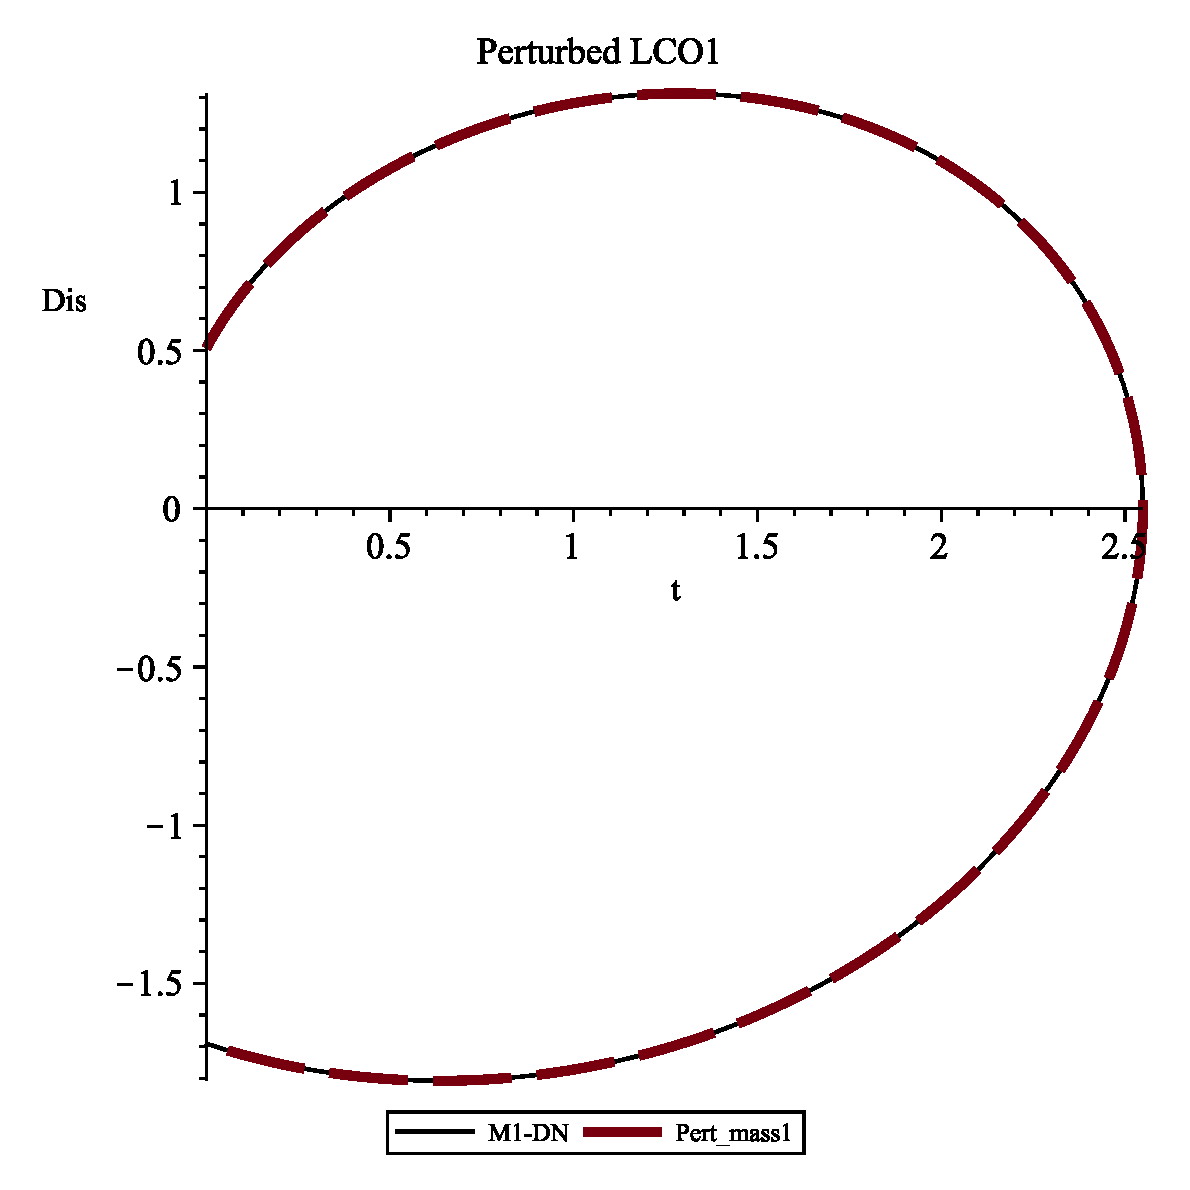
\includegraphics[width= 0.5 \linewidth]{1BoundaryConditions_Method3plot2d32.eps}}
	\subfloat[Second DOF]{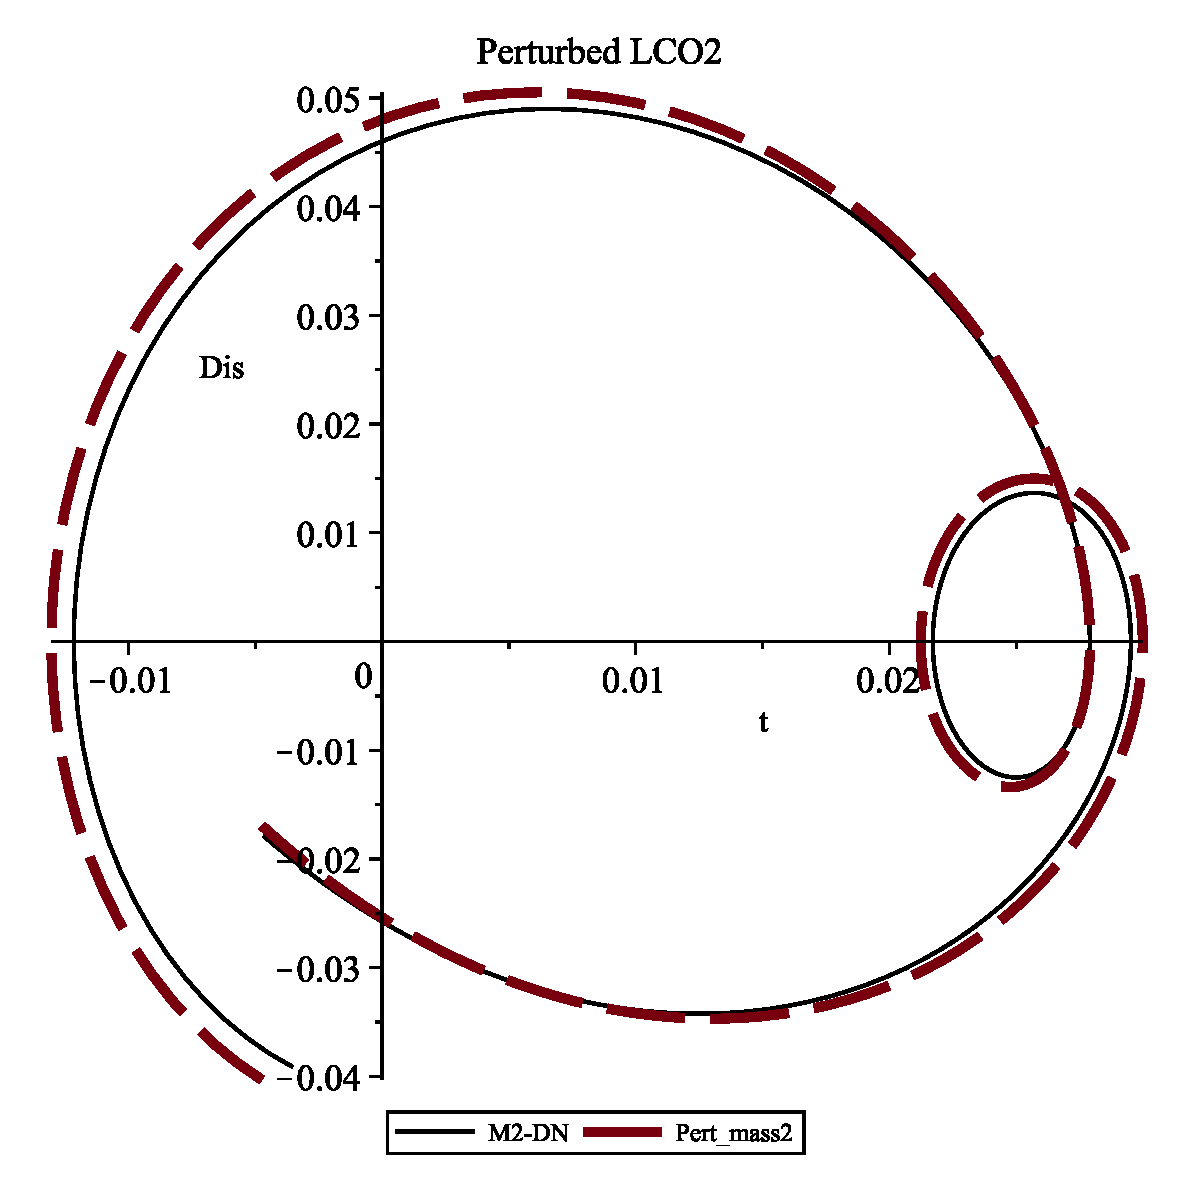
\includegraphics[width= 0.5 \linewidth]{1BoundaryConditions_Method3plot2d34.eps}}
	\caption{Comparison between DN and ANA results:$\epsilon=0.01,T_p=4.7883398,T_0=4.74997,T_{DN}=4,7885159$}
\end{figure}

\begin{figure}[h]
	\subfloat[First DOF]{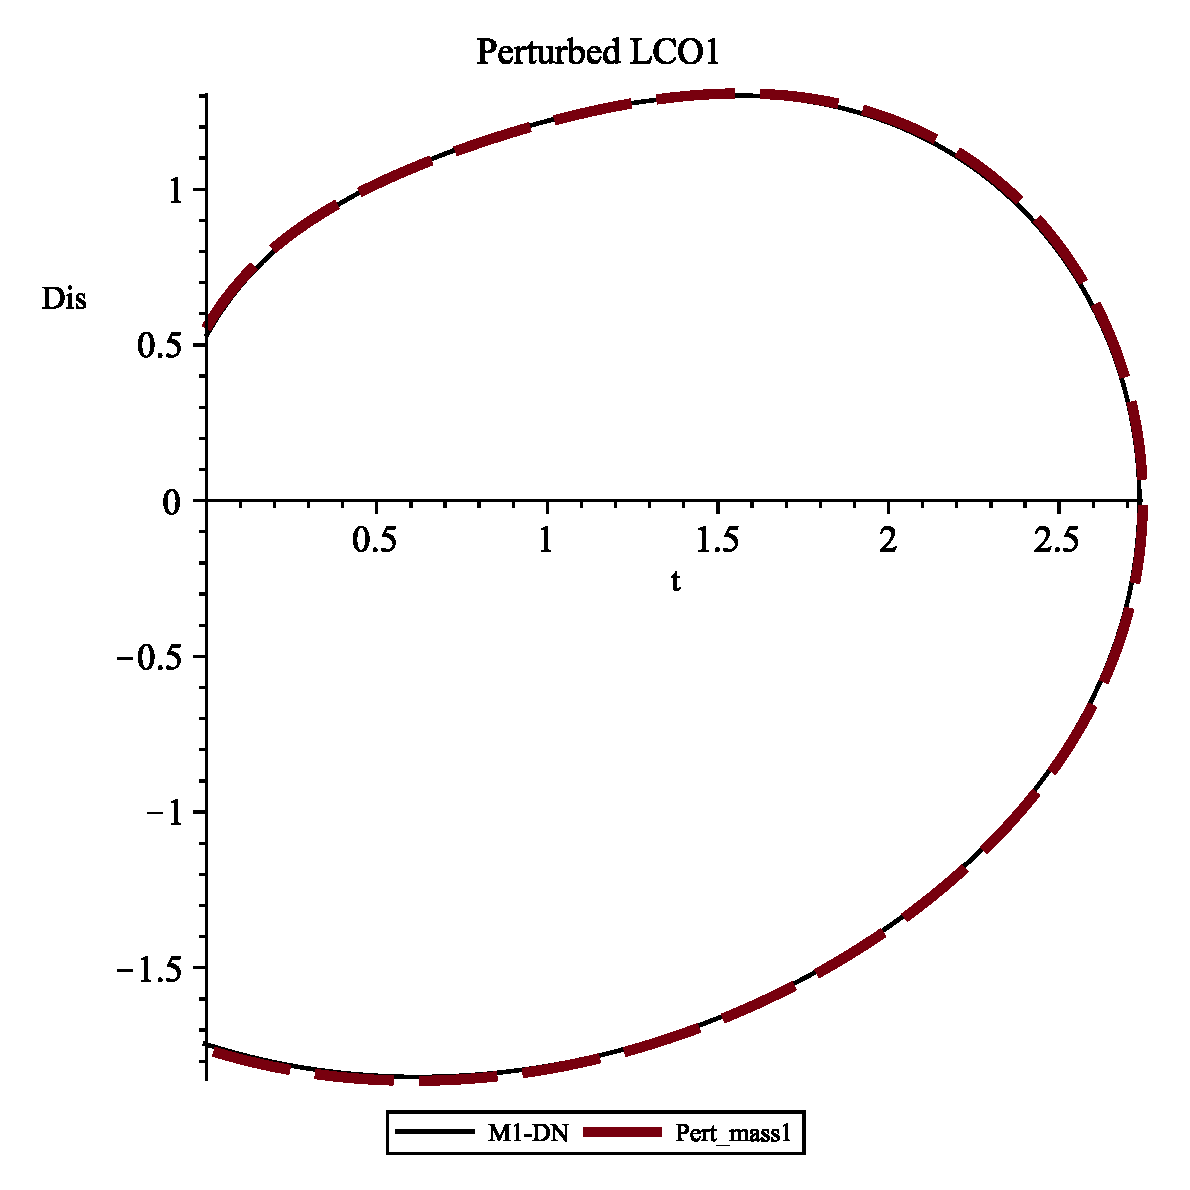
\includegraphics[width= 0.5 \linewidth]{3BoundaryConditions_Method3plot2d32.eps}}
	\subfloat[Second DOF]{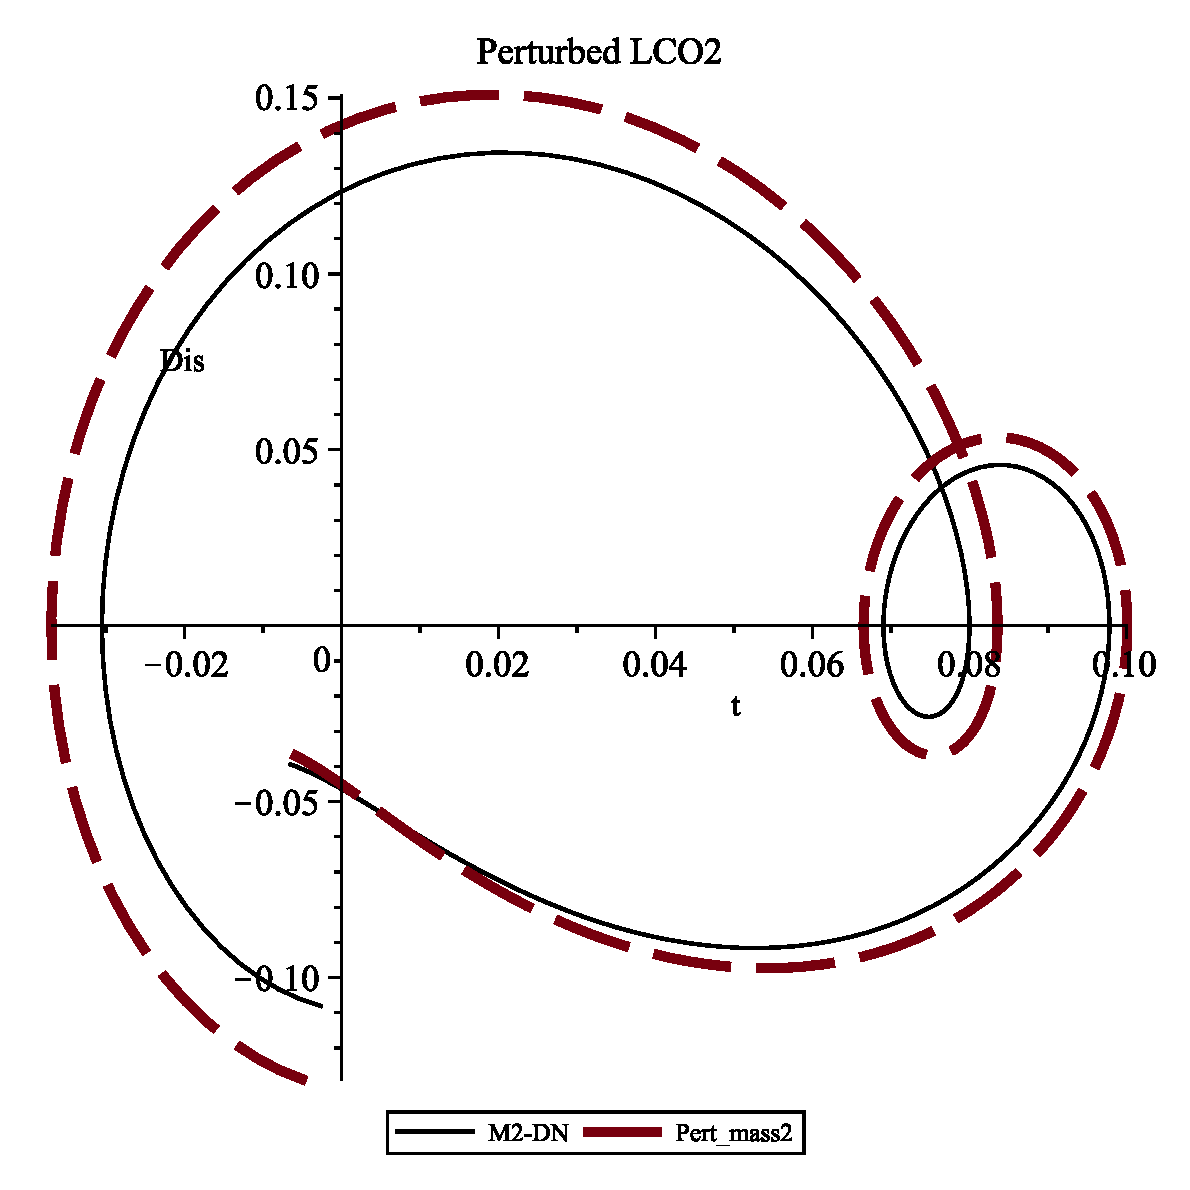
\includegraphics[width= 0.5 \linewidth]{3BoundaryConditions_Method3plot2d34.eps}}
	\caption{Comparison between DN and ANA results:$\epsilon=0.03,T_p=5.06612,T_0=4.74997,T_{DN}=5.0889$}
\end{figure}

\begin{figure}[h]
	\subfloat[First DOF]{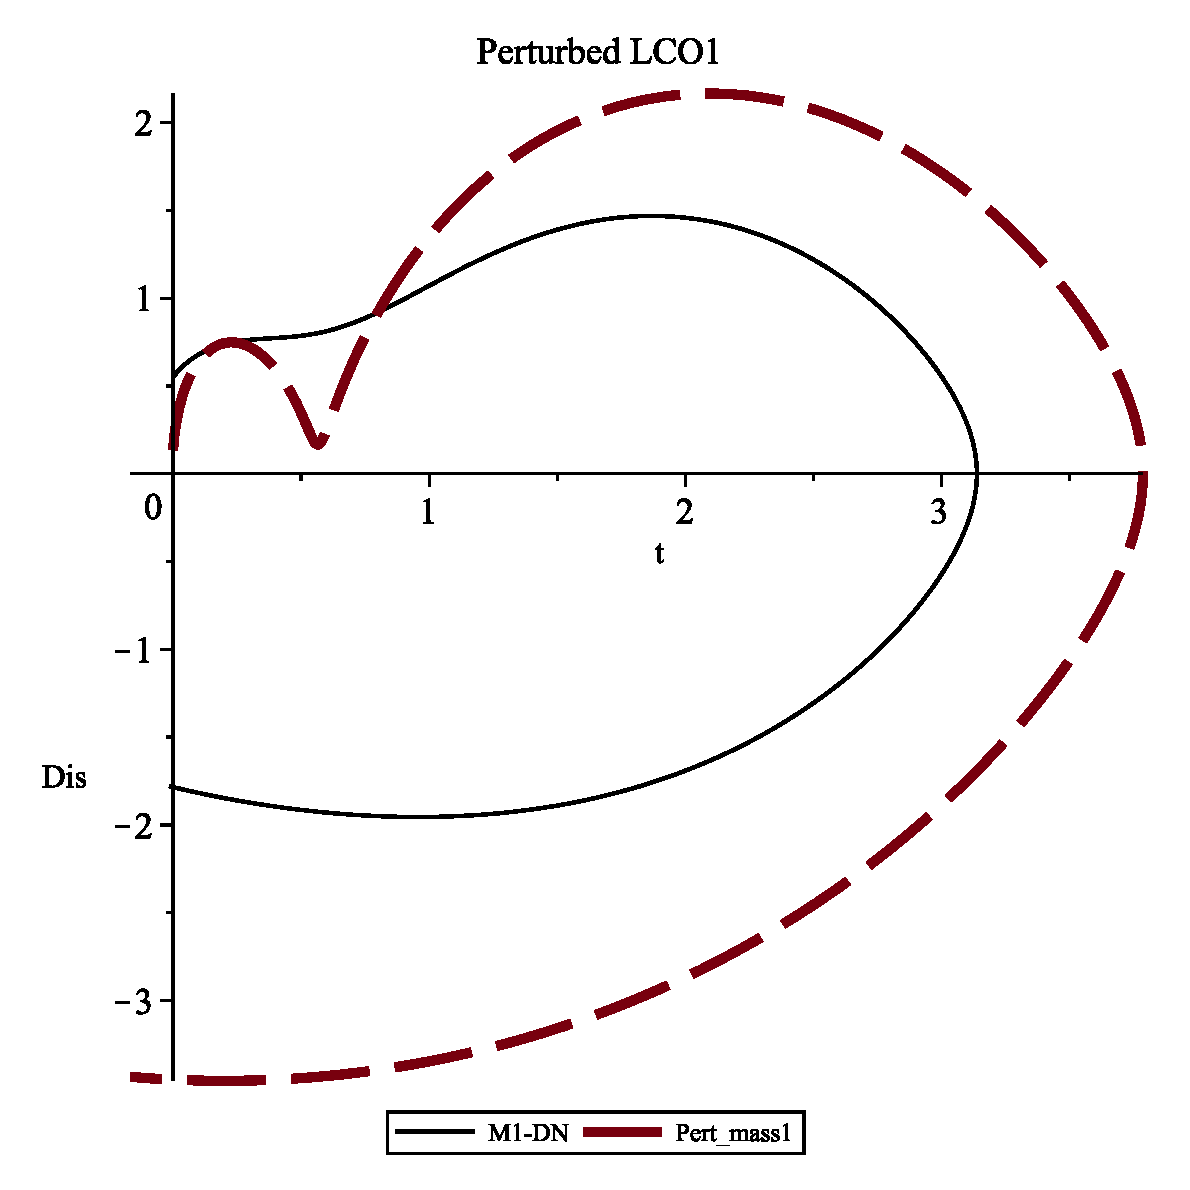
\includegraphics[width= 0.5 \linewidth]{5BoundaryConditions_Method3plot2d32.eps}}
	\subfloat[Second DOF]{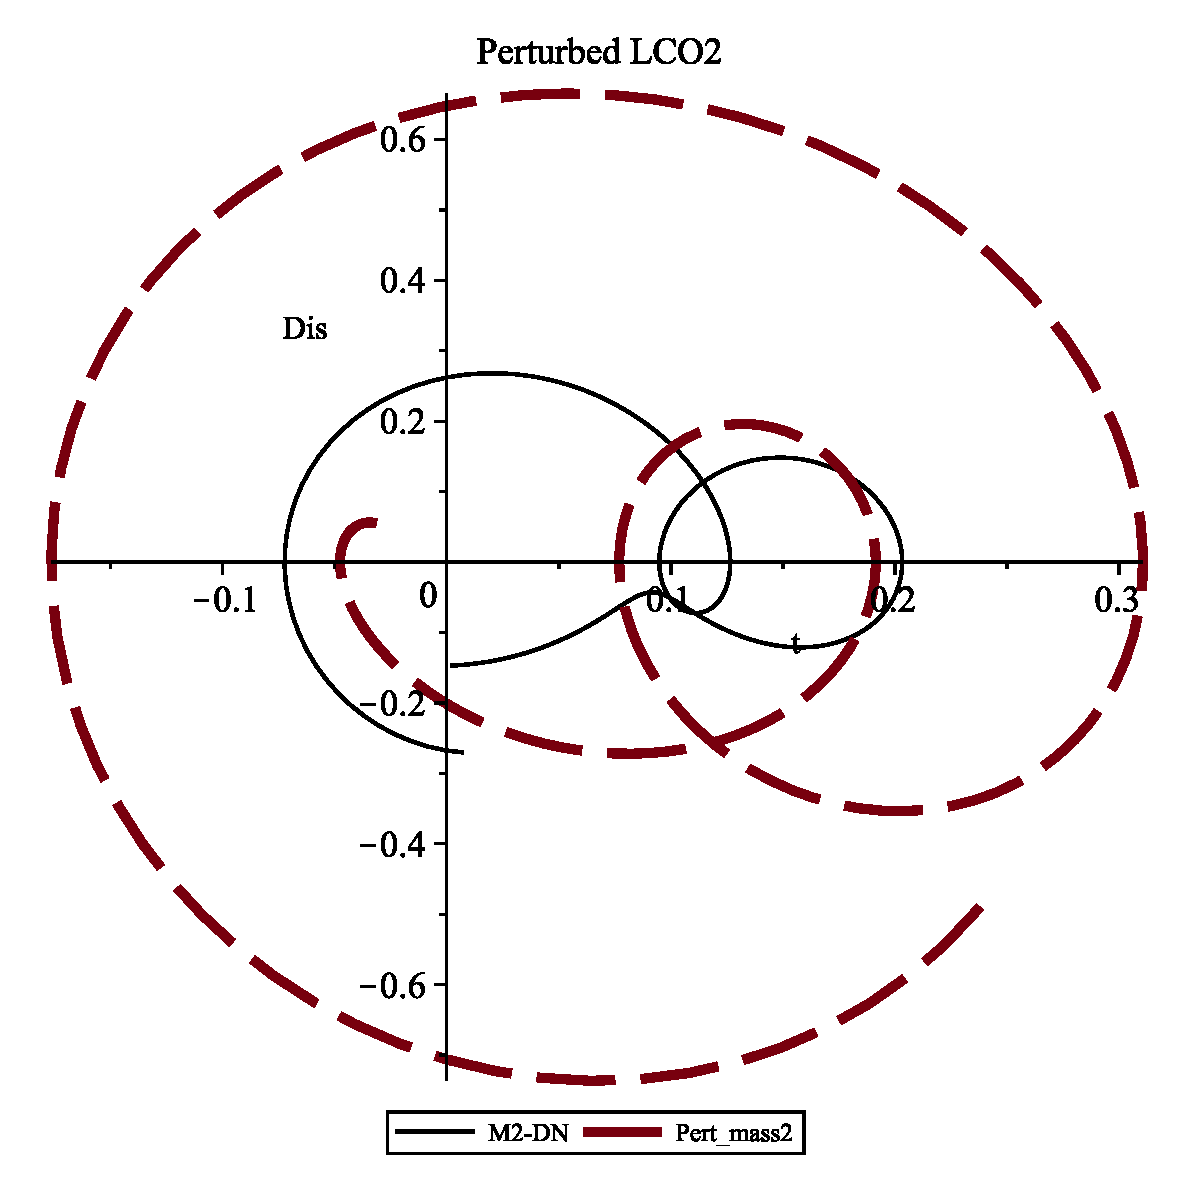
\includegraphics[width= 0.5 \linewidth]{5BoundaryConditions_Method3plot2d34.eps}}
	\caption{Comparison between DN and ANA results:$\epsilon=0.05,T_p=5.86293,T_0=4.74997,T_{DN}=5.876609$}
\end{figure}
It still fails when the $\epsilon$ gets bigger, even with higher orders' correction terms. 


\subsection{work flow}
First, use the boundary conditions to get the first order correction function with undefined coefficients, use the boundary conditions to solve them. Then get full solution using iteration scheme.
\clearpage
\bibliographystyle{alpha}
\bibliography{sample}

\end{document}